\documentclass[11pt, oneside, numbers=noenddot]{scrbook}   		% Allgemeine Schriftgröße, Dokumententyp
\input{./includes/htl_definintions.tex}		% Formatierung der Dokuments, Diverse Befehle


%	########################################################
% 					Allgemeine Informationen			
%	########################################################

% Titel der Arbeit:
\def\htlArbeitsthema{sunnyHOME}	

%	########################################################

\begin{document}

%	########################################################
% 						Einleitung			
%	########################################################
\pagenumbering{roman}	% Beginn mit römischen Seitenzahlen

%	--------------------------------------------------------
% 	Deckblatt
%	--------------------------------------------------------			
% !TEX root = ../Vorlage_DA.tex

%	########################################################
% 							Deckblatt
%	########################################################


\titlehead{%
\vspace{-4em}\centering \includegraphics[width=0.15\textwidth]{./includes/htl_c_cmyk_rein.pdf}\\[3ex]
Höhere Technische Bundeslehranstalt\\
und Bundesfachschule\\
im Hermann Fuchs Bundesschulzentrum
}
\title{\vspace{4em}\htlArbeitsthema}
\subtitle{ {\Large Diplomarbeit}\\[1em]Schulautonomer Schwerpunkt Communications}
\author{\\[3.5em] 
\emph{ausgeführt im Schuljahr 2018/2019 von:} \\[1em] 
Andreas Herz, 5BHELS\\[4em]
\emph{Betreuer:} \\[1em]
 Dipl.-Ing. Roland Sageder
}
\date{\vspace{3\baselineskip}\today}

\begin{titlepage}	
\maketitle
\end{titlepage}


%	--------------------------------------------------------
% 	Arbeitstitel
%	--------------------------------------------------------		
% !TEX root = ../Vorlage_DA.tex
%	########################################################
% 							Arbeitstitel
%	########################################################


%	--------------------------------------------------------
% 	Überschrift, Inhaltsverzeichnis
%	--------------------------------------------------------
\chapter*{Thema: \newline \htlArbeitsthema }



%	--------------------------------------------------------
% 	Bearbeiter
%	--------------------------------------------------------
\section*{Subthemen und Bearbeiter:}


\textbf{Umweltdatenerfassung}\\ 
Andreas Herz, 5BHELS\\
\emph{Betreuer:} Dipl.-Ing. Roland Sageder\\[2ex] 
%
\textbf{Basisstation}\\ 
Andreas Herz, 5BHELS\\
\emph{Betreuer:} Dipl.-Ing. Roland Sageder\\[2ex] 




%--------------------------------------------------------------------------------
%  Vorgeschriebene Dokumentationsseiten
%--------------------------------------------------------------------------------

\pagebreak
\thispagestyle{empty}
\newgeometry{top=2cm, bottom=1.5cm}

\begin{minipage}[c]{0.20\linewidth}
\includegraphics[width=0.8\linewidth]{media/images/htl_c_cmyk_rein}
\end{minipage}
\begin{minipage}[c]{0.6\linewidth}
\begin{center}
{\bfseries\sffamily\large Höhere  technische  Bundeslehranstalt\\
und  Bundesfachschule  Braunau\\
Elektronik und Technische Informatik\\
{\normalsize Schulautonomer Schwerpunkt Communications} }
\end{center}
\end{minipage}
\begin{minipage}[c]{0.2\linewidth}
\hfill \includegraphics[width=0.8\linewidth]{media/images/htl-bildung-mit-zukunft}
\end{minipage}\\

\vspace{1em}
\begin{center}
\bfseries\sffamily\Large
DIPLOMARBEIT DOKUMENTATION
\end{center}
\vspace{1ex}

\renewcommand{\arraystretch}{2}
\begin{tabularx}{1\textwidth}{ p{3.5cm} X }

\textbf{Verfasser/innen} & 
Andreas Herz \\

\textbf{Jahrgang\linebreak Schuljahr} & 
5BHELS 2018/2019 \\

\textbf{\mbox{Thema der} \mbox{Diplomarbeit}} & 
\htlArbeitsthema \\

\textbf{Aufgabenstellung} & 
{Die Aufgabenstellung war, eine Energie-autarke Wetterstation zu entwickeln. Es sollen verschiedene Sensoren, wie zum Beispiel Niederschlags- oder UV-Sensoren verwendet werden. Die Daten der Sensoren sollen dann über einen Mikrocontroller eingelesen und an einen Web-Server gesendet werden. Dieser wertet diese Daten aus, welche dann über eine Website oder eine App visualisiert werden.} \\

\textbf{Realisierung} & 
{Realisiert wird das Projekt mithilfe des ESP32 Mikrocontrollers. Dieser hat die benötigte Energie-Effizienz und lässt sich leicht an verschiedenste Sensoren anbinden. Mit Hilfe eines GPS-Receivers soll der Standort der Wetterstation bestimmt werden, und mit Hilfe von Solarzellen, soll das ganze System Energie-autark realisiert werden. } \\

\textbf{Ergebnisse} & 
{Die wichtigsten Ergebnisse sollen sein:
    \begin{itemize}
        \item Konzept fertiggestellt 
        \item Sensoren können messen
        \item GPS-Signal wird empfangen
        \item Datenübertragung funktioniert
        \item Visualisierung funktioniert
        \item Energie-Versorgung funktioniert
        \item Diplomarbeit verfasst 
    \end{itemize}
} \\

\end{tabularx}

%--------------------------------------------------------------------------------

\pagebreak
\thispagestyle{empty}
\newgeometry{top=2cm, bottom=1.5cm}

\begin{minipage}[c]{0.20\linewidth}
\includegraphics[width=0.8\linewidth]{media/images/htl_c_cmyk_rein}
\end{minipage}
\begin{minipage}[c]{0.6\linewidth}
\begin{center}
{\bfseries\sffamily\large Höhere  technische  Bundeslehranstalt\\
und  Bundesfachschule  Braunau\\
Elektronik und Technische Informatik\\
{\normalsize Schulautonomer Schwerpunkt Communications} }
\end{center}
\end{minipage}
\begin{minipage}[c]{0.2\linewidth}
\hfill \includegraphics[width=0.8\linewidth]{media/images/htl-bildung-mit-zukunft}
\end{minipage}\\

\vspace{1em}

\renewcommand{\arraystretch}{2}
\begin{tabularx}{1\textwidth}{ p{3.5cm} X }

\textbf{\mbox{Typische Grafik,} \mbox{Foto etc.} \mbox{(mit Erläuterung)}} & 
{
Die Wetterstation sunnyHOME:
\begin{center}
	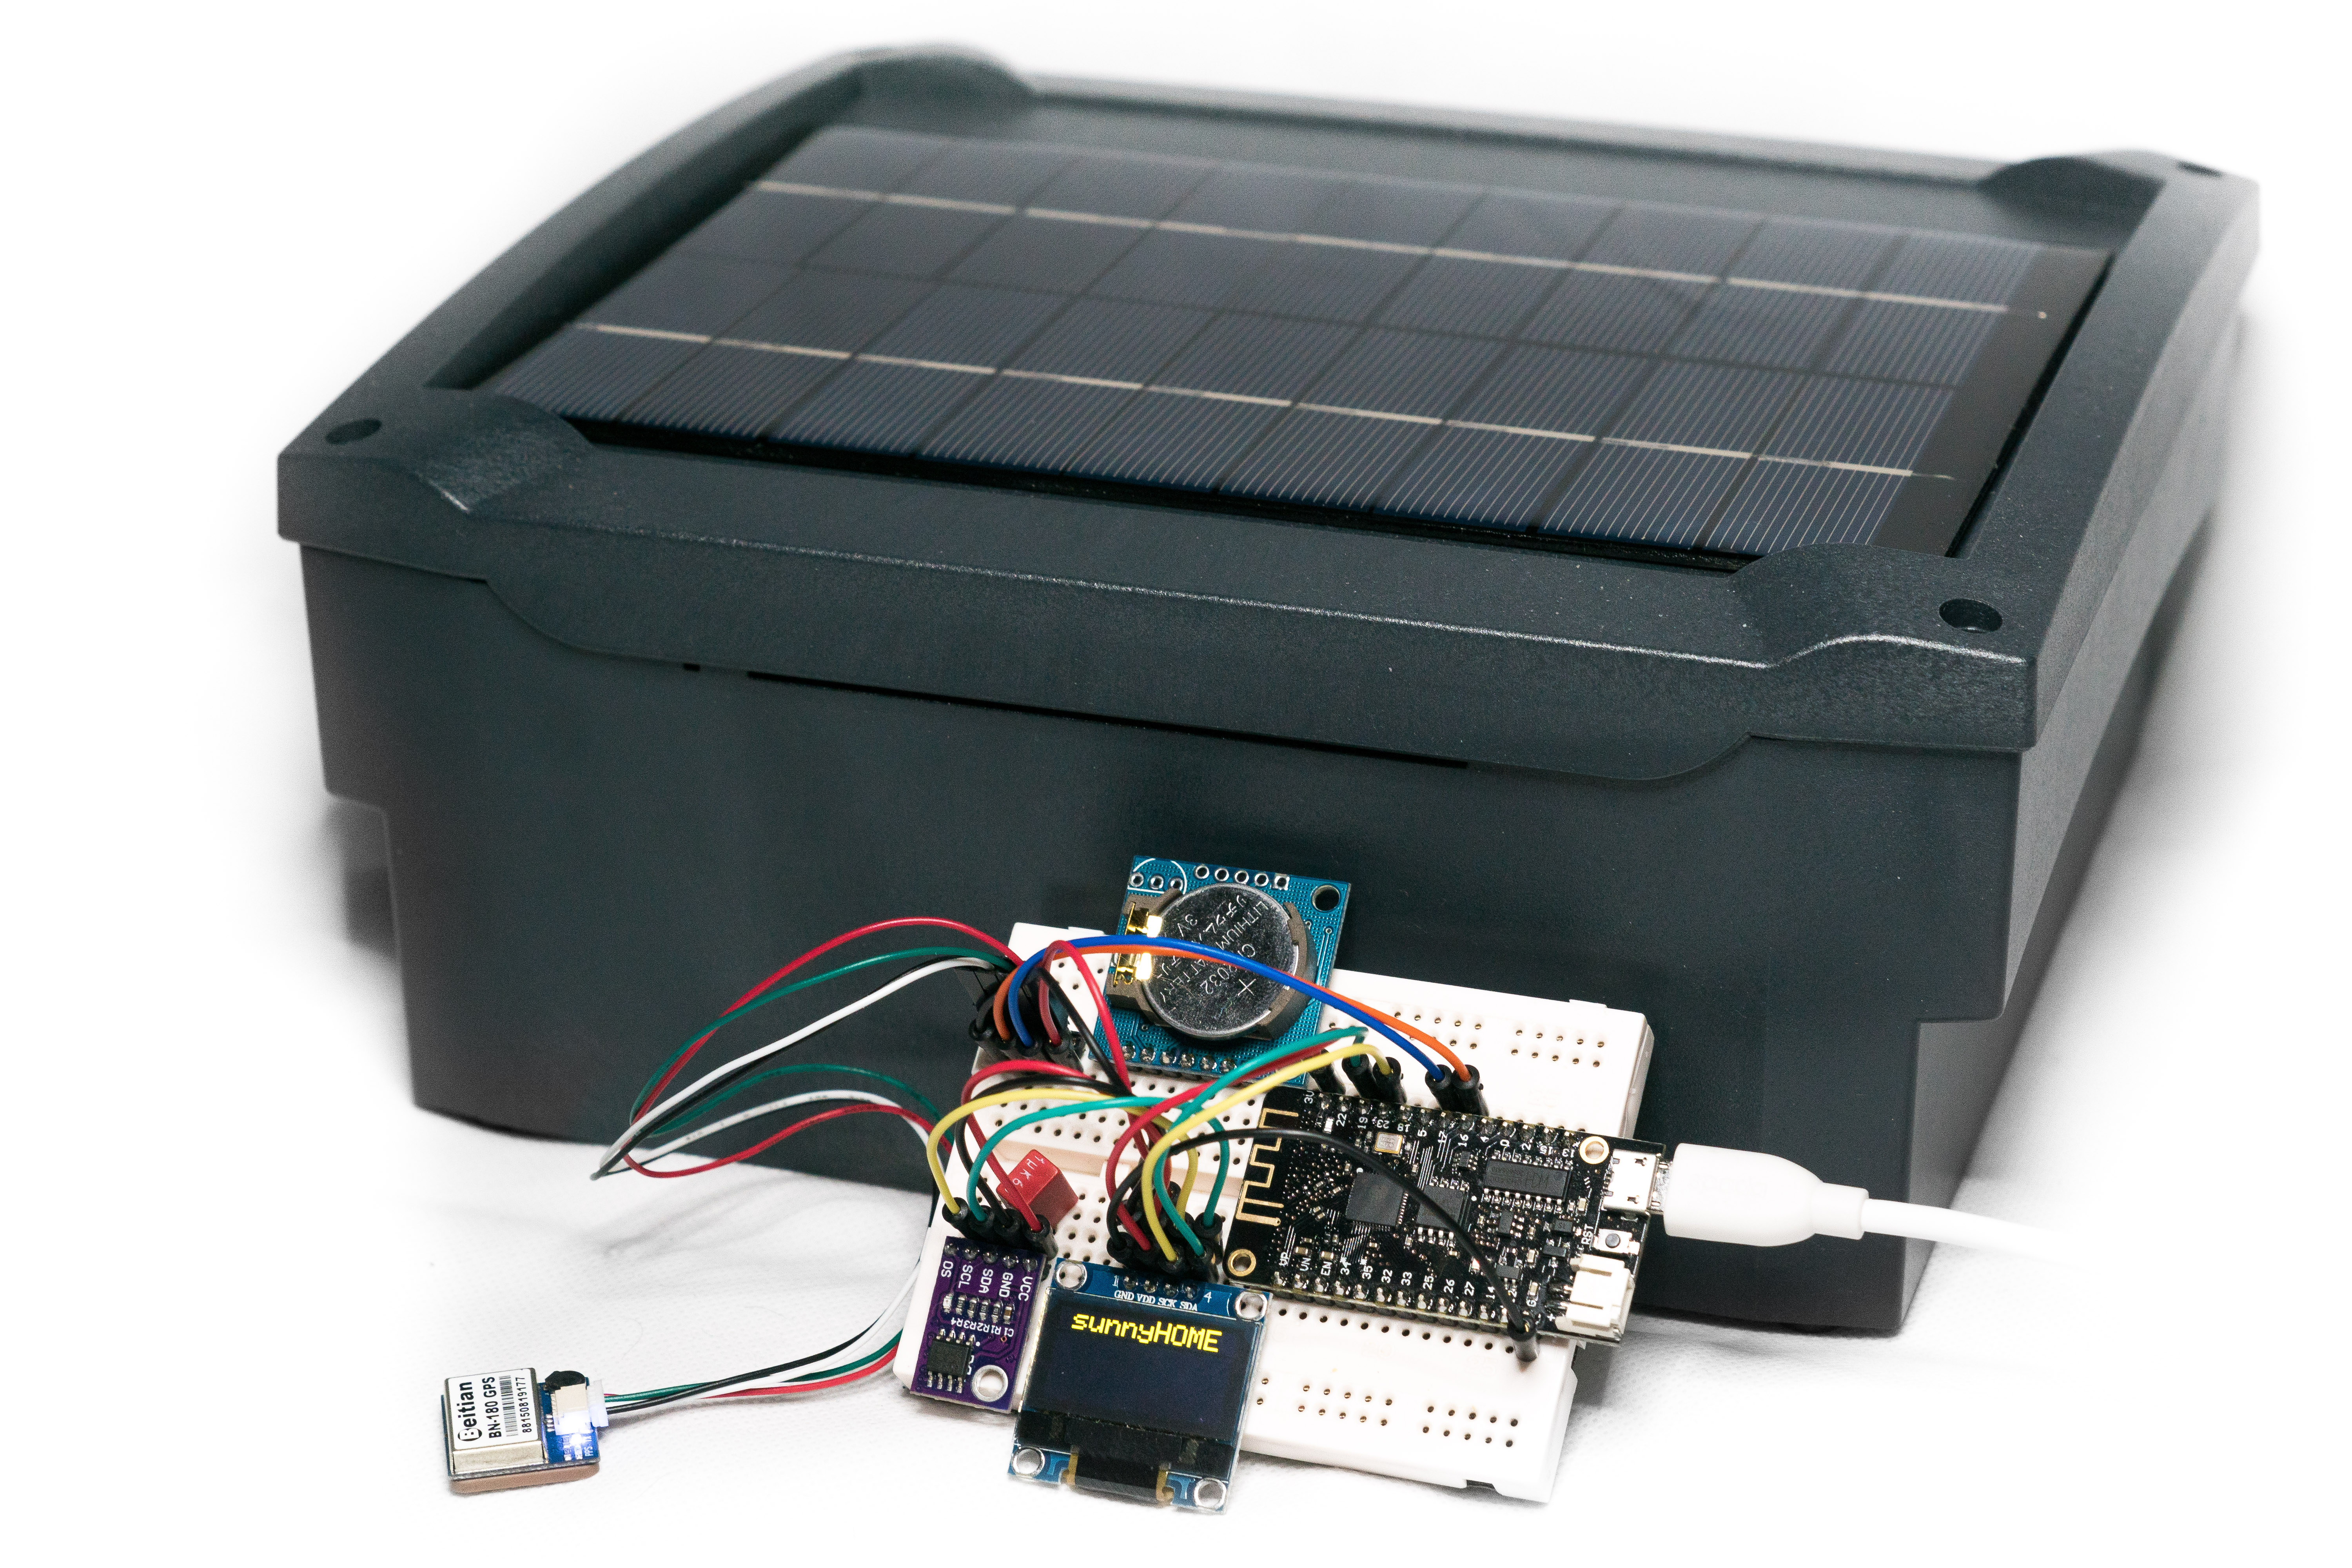
\includegraphics[width=1\linewidth]{media/images/sunnyHOME.jpg}
\end{center}
} \\


\textbf{\mbox{Möglichkeiten der} Einsichtnahme \mbox{in die Arbeit}} & 
{Archiv der HTL Braunau, bzw.\newline \url{https://diplomarbeiten.berufsbildendeschulen.at/}} \\


\end{tabularx}




%--------------------------------------------------------------------------------
% Unterschriften
%--------------------------------------------------------------------------------


\vspace*{\fill}

\textbf{Approbation (Datum / Unterschrift)}

\fbox{
\begin{minipage}[t][3cm]{0.5\linewidth}
Prüfer/Prüferin: \\
%\hspace*{\fill}\includegraphics[width=0.8\linewidth]{fig/Unterschrift}\hspace*{\fill}
\vfill
\end{minipage}}
\fbox{
\begin{minipage}[t][3cm]{0.5\linewidth}
Direktor/Direktorin
\\ Abteilungsvorstand/Abteilungsvorständin
\vfill
\end{minipage}
}

%--------------------------------------------------------------------------------


%--------------------------------------------------------------------------------
%  Vorgeschriebene Dokumentationsseiten (Englisch)
%--------------------------------------------------------------------------------

\pagebreak
\thispagestyle{empty}
\newgeometry{top=2cm, bottom=1.5cm}

\begin{minipage}[c]{0.20\linewidth}
\includegraphics[width=0.8\linewidth]{media/images/htl_c_cmyk_rein}
\end{minipage}
\begin{minipage}[c]{0.6\linewidth}
\begin{center}
{\bfseries\sffamily\large HTBLA Braunau/Inn\\
COLLEGE of ENGINEERING\\
Dept. Elektronik und Technische Informatik\\
{\normalsize Educational focus Communications} }
\end{center}
\end{minipage}
\begin{minipage}[c]{0.2\linewidth}
\hfill \includegraphics[width=0.8\linewidth]{media/images/htl-bildung-mit-zukunft}
\end{minipage}\\

\vspace{1em}
\begin{center}
\bfseries\sffamily\Large
DIPLOMA THESIS Documentation
\end{center}
\vspace{1ex}

\renewcommand{\arraystretch}{2}
\begin{tabularx}{1\textwidth}{ p{3.5cm} X }

\textbf{Author(s)} & 
Andreas Herz \\


\textbf{Form \mbox{Academic year}} & 
5BHELS 2018/2019 \\

\textbf{Topic} & 
\htlArbeitsthema \\

\textbf{Assignment \mbox{of tasks}} & 
{The major task was to develope a self-sufficient weather station. Various sensors should be used,  like for example rainfall- and UV-sensors. The measured data should be read from the ESP32, and then published to a web-server. The web-server evaluates this data, which then will be visualized via a website or a mobile application.} \\

\textbf{Realisation} & 
{The realisation will happen with help of the ESP32 microcontroller. The ESP32 has the needed energy-efficiancy and can be easily connected to a wide variety of sensors. A GPS-receiver should provide the current location of the weather station, and solar cells should  keep the system self-sufficient.} \\

\textbf{Results} & 
{The most important results should be:
    \begin{itemize}
        \item concept is done
        \item sensors are able to measure
        \item receiving the GPS-signal
        \item transfering of data works
        \item visualization works
        \item power-supply works
        \item diploma thesis is written 
    \end{itemize}} \\

    \end{tabularx}

%--------------------------------------------------------------------------------

\pagebreak
\thispagestyle{empty}
\newgeometry{top=2cm, bottom=1.5cm}


\begin{minipage}[c]{0.20\linewidth}
\includegraphics[width=0.8\linewidth]{media/images/htl_c_cmyk_rein}
\end{minipage}
\begin{minipage}[c]{0.6\linewidth}
\begin{center}
{\bfseries\sffamily\large HTBLA Braunau/Inn\\
COLLEGE of ENGINEERING\\
Dept. Elektronik und Technische Informatik\\
{\normalsize Educational focus Communications} }
\end{center}
\end{minipage}
\begin{minipage}[c]{0.2\linewidth}
\hfill \includegraphics[width=0.8\linewidth]{media/images/htl-bildung-mit-zukunft}
\end{minipage}\\

\vspace{1em}

\renewcommand{\arraystretch}{2}
\begin{tabularx}{1\textwidth}{ p{3.5cm} X }

\textbf{\mbox{Illustrative graph,} \mbox{photo} \mbox{(incl. explanation)}} & 
{
The sunnyHOME weather station:
\begin{center}
	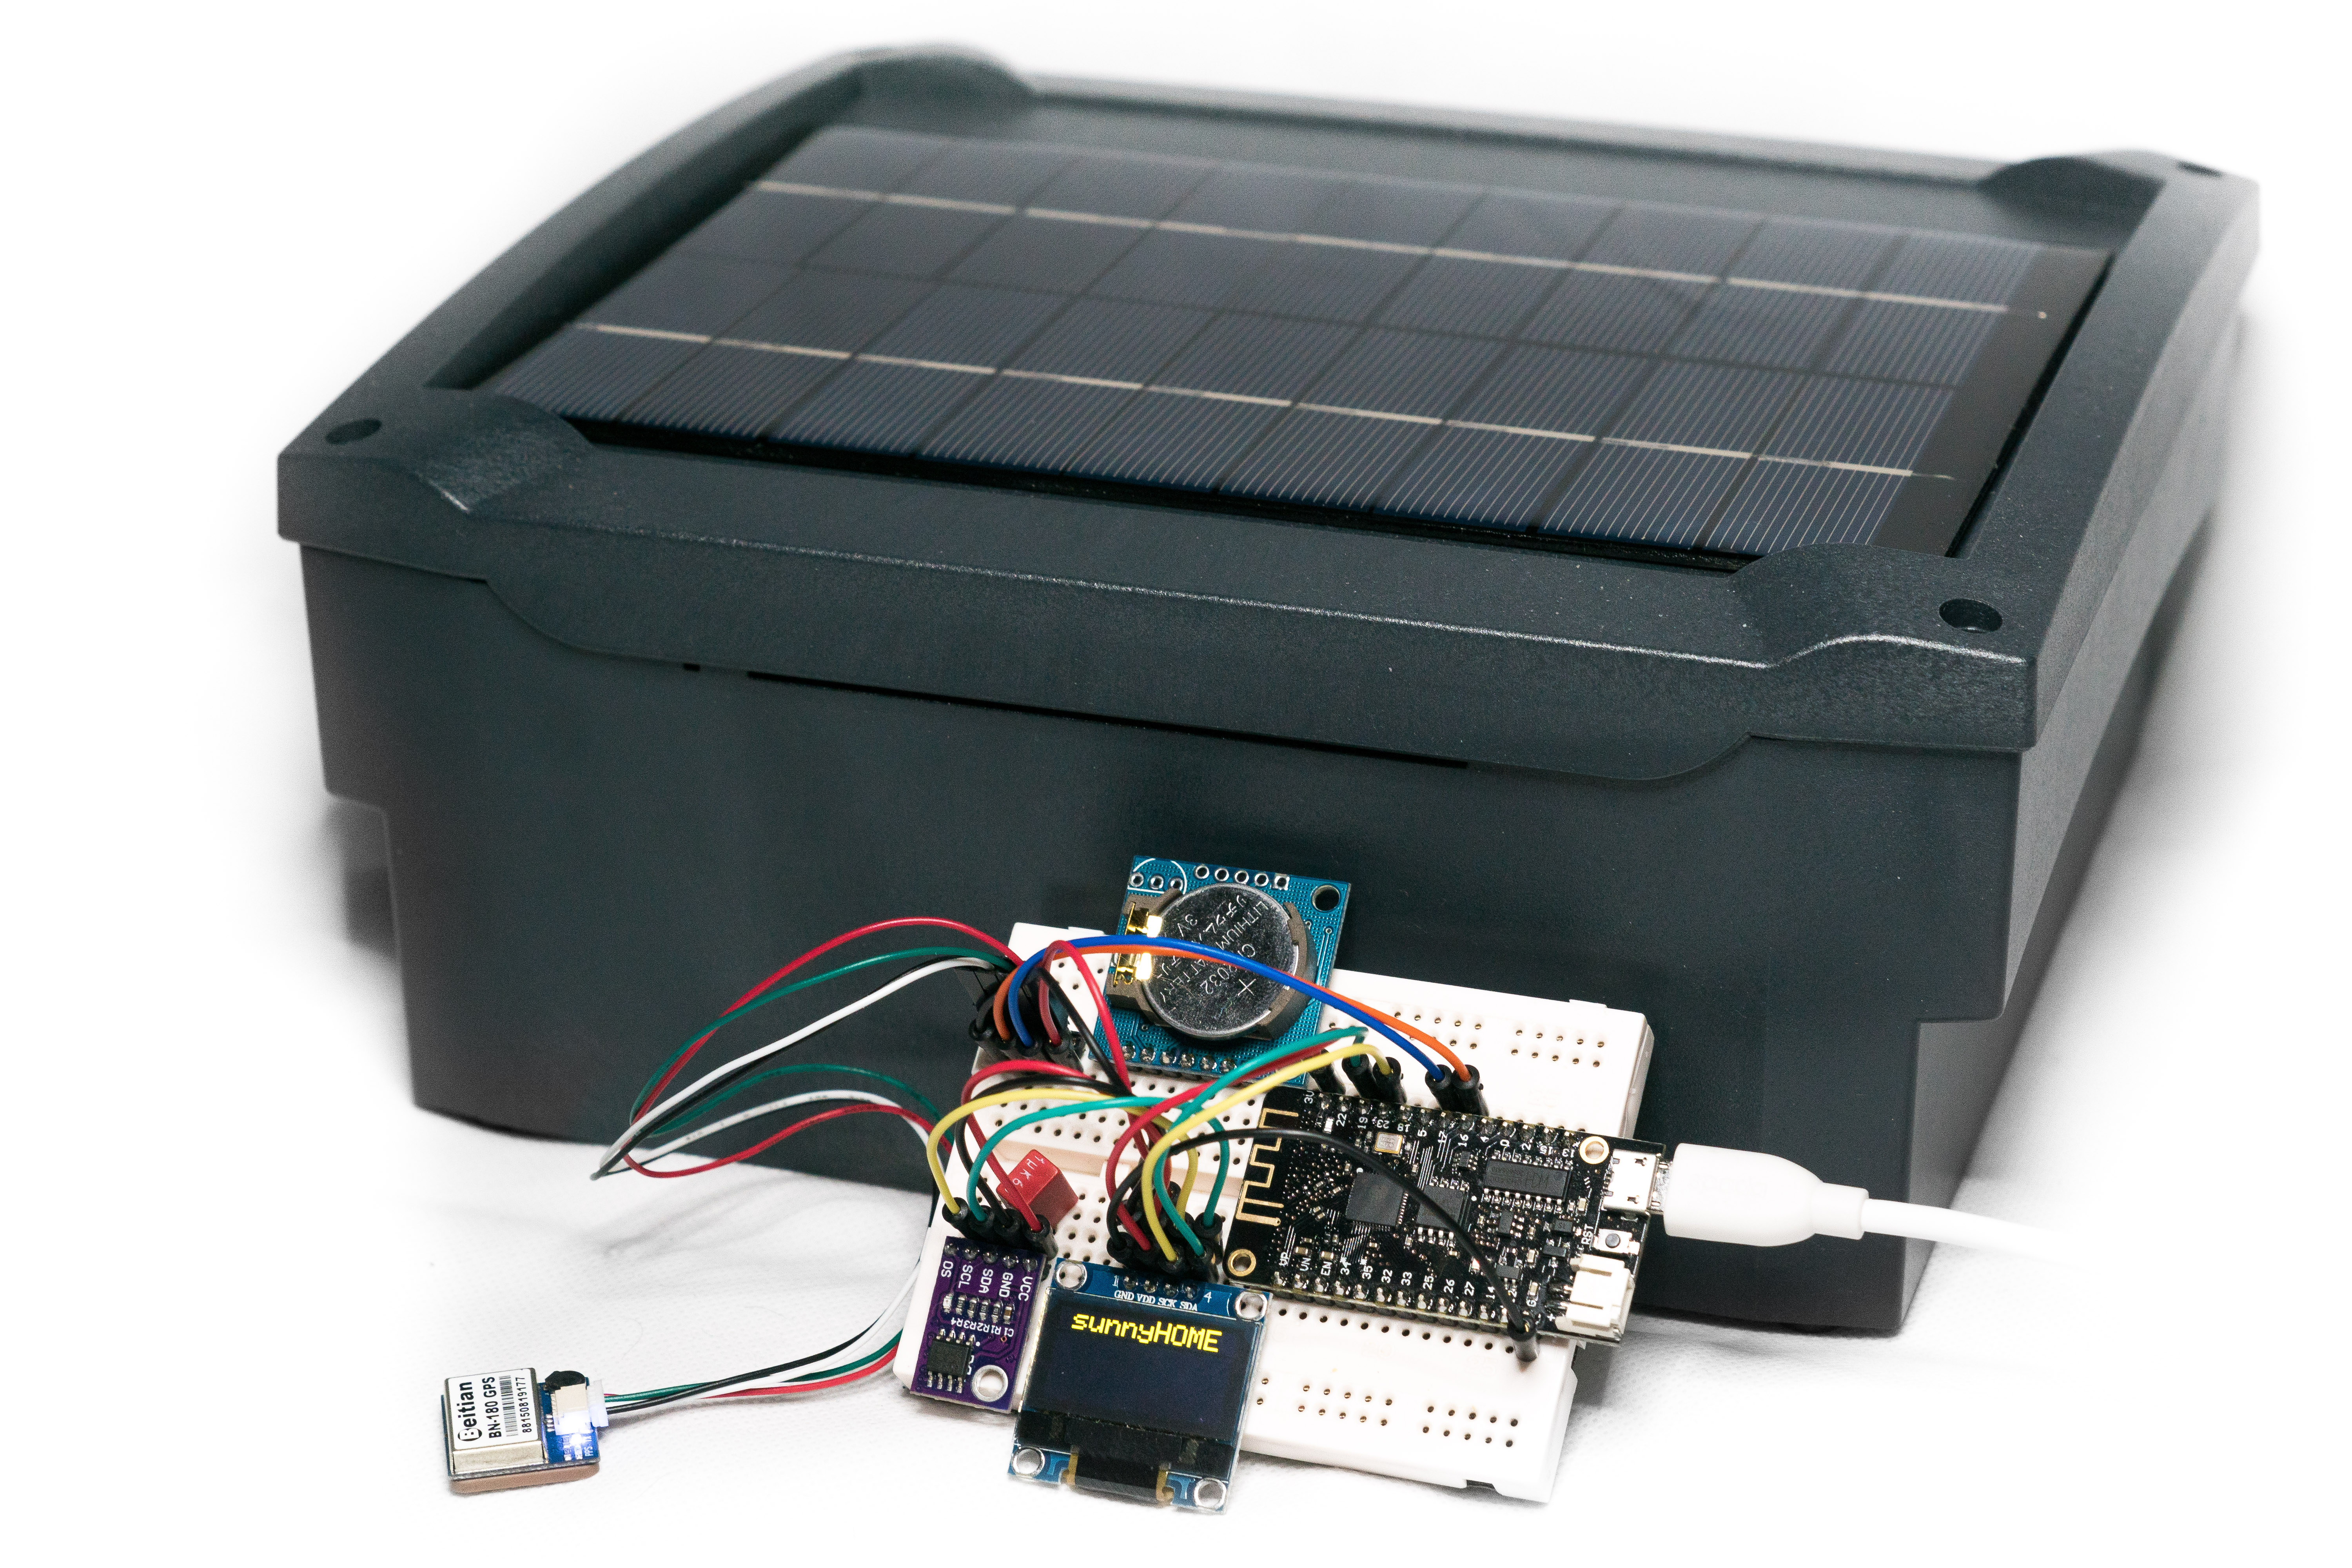
\includegraphics[width=1\linewidth]{media/images/sunnyHOME.jpg}
\end{center}
} \\

\textbf{\mbox{Accessibility of} \mbox{diploma thesis}} & 
{HTL Braunau archive, or\newline \url{https://diplomarbeiten.berufsbildendeschulen.at/}} \\



\end{tabularx}




%--------------------------------------------------------------------------------
% Unterschriften
%--------------------------------------------------------------------------------


\vspace*{\fill}

\textbf{Approval (date / signature)}

\fbox{
\begin{minipage}[t][3cm]{0.5\linewidth}
\centering
Examiner \\
%\hspace*{\fill}\includegraphics[width=0.8\linewidth]{fig/Unterschrift}\hspace*{\fill}
\vfill
\end{minipage}}
\fbox{
\begin{minipage}[t][3cm]{0.5\linewidth}
\centering
Head of College / Department
\vfill
\end{minipage}
}

%--------------------------------------------------------------------------------

\restoregeometry



%	--------------------------------------------------------
% 	Eidesstattliche Erklärung
%	--------------------------------------------------------			
\input{./chapters/03-Erklaerung.tex}

%	--------------------------------------------------------
% 	Inhaltsverzeichnis
%	--------------------------------------------------------			
\tableofcontents

%	--------------------------------------------------------
% 	Vorwort
%	--------------------------------------------------------	
% !TEX root = ../Vorlage_DA.tex
%	########################################################
% 							Vorwort
%	########################################################


%	--------------------------------------------------------
% 	Überschrift, Inhaltsverzeichnis
%	--------------------------------------------------------
\chapter*{Vorwort}
\addcontentsline{toc}{chapter}{Vorwort}


%	--------------------------------------------------------
% 	Inhalt
%	--------------------------------------------------------
Sehr geehrte Damen und Herren, liebe Leserschaft, \newline


vor Ihnen findet sich eine Diplomarbeit zum Thema „sunnyHOME – Umweltdatenerfassung“, welche von dem HTL-Braunau Schüler Andreas Herz verfasst wurde. Dieser besuchte an der HTL Braunau den schulautonomen Zweig „Communications“, und schieb auf Grund des Abschlusses die vor Ihnen liegende Diplomarbeit.\newline

Ende des letzten Schuljahres (2017/18), entschloss ich mich (Andreas Herz), mit einem Klassenkameraden, die Themenstellung einer Energie-autarken Wetterstation in Angriff zu nehmen. Da dieser Klassenkamerad jedoch kurzfristig nicht mehr aufsteigen durfte, wurde das Projekt zu einer Einzelarbeit.\newline

Mit Hilfe von DI. Roland Sageder, welcher der zugewiesene Betreuer des Projektes war, konnten wir uns bereits vor den Sommerferien ein grobes Bild des Vorhabens machen. Auch wenn in den Sommerferien 2018 recherchiert wurde, mussten nach der vorgezogenen Matura die Pläne, auf Grund der plötzlichen Einzelarbeit, verändert werden. Das Projekt musste auf die Grundfunktionen begrenzt werden, und Zeitpläne wurden erstellt. Frau Margit Fuchs, welche zur Aushilfe beim Projektmanagement zugeteilt war, half mir mit guten Vorschlägen dabei. Während des Jahres wurde aber immer wieder klar, dass man für Softwareprojekte oft mehr Zeit braucht als angesetzt ist. Immer wieder gab es Hindernisse und Pannen, in welchen ich mir zusätzliches Wissen aneignen musste um weiterzukommen. Im Endeffekt sehe ich dann jedoch ein, dass jede Panne eine lehrreiche Lektion war.\newline

Hiermit möchte ich die Gelegenheit nutzen, um meinen Dank an all diejenigen auszusprechen, die mir bei meinem Projekt geholfen haben. Insbesondere möchte ich dem Herrn Dipl. Ing. Roland Sageder danken. Für seine Geduld mit mir, in Situationen in denen ich vielleicht etwas mehr als nur einmal eine Erklärung gebraucht habe und auch die Motivation, welche er mir immer wieder gegeben hat. Aber auch Frau Margit Fuchs möchte ich danken. Ohne sie hätte ich das Projekt definitiv nicht so gut organisieren können. \newline

Ich wünsche Ihnen nun viel Freunde beim Lesen dieser Abschlussarbeit.\newline

Andreas Herz 
\newline
\newline 4963 St. Peter am Hart, \today


%	--------------------------------------------------------
% 	Zusammenfassung
%	--------------------------------------------------------		
% !TEX root = ../Vorlage_DA.tex
%	########################################################
% 							Zusammenfassung
%	########################################################


%	--------------------------------------------------------
% 	Überschrift, Inhaltsverzeichnis
%	--------------------------------------------------------
\chapter*{Kurzfassung}
\addcontentsline{toc}{chapter}{Kurzfassung}



%	--------------------------------------------------------
% 	Inhalt
%	--------------------------------------------------------
In dieser Diplomarbeit geht es hauptsächlich um die Arduino-Programmierung eines ESP32 im Zusammenhang mit IoT (Internet of Things) und Energy-Harvesting. Für den Endbenutzer soll eine Wetterstation geschaffen werden, welche robust, unabhängig von einer Stromversorgung und leicht zu modifizieren ist. 

„sunnyHOME“ ist ein Gerät, welches Wetterdaten sammelt und kabellos ins Internet publiziert. Es können verschiedene Sensoren, wie zum Beispiel Niederschlags- oder UV-Sensoren, verwendet werden. Die Daten der Sensoren werden dann über einen Mikrocontroller eingelesen und an einen Web-Server gesendet. Dieser wertet die Daten aus, welche dann über eine Website oder eine App visualisiert werden. Somit kann man von überall auf der Welt nachschauen, ob zum Beispiel die Blumen im Garten genug Wasser bekommen oder nicht.   



%	--------------------------------------------------------
% 	Abstract
%	--------------------------------------------------------		
% !TEX root = ../Diplomarbeit_sunnyHOME.tex
%	########################################################
% 							Abstract
%	########################################################


%	--------------------------------------------------------
% 	Überschrift, Inhaltsverzeichnis
%	--------------------------------------------------------
\chapter*{Abstract}
\addcontentsline{toc}{chapter}{Abstract}



%	--------------------------------------------------------
% 	Inhalt
%	--------------------------------------------------------
This diploma thesis focuses on the Arduino programming of an ESP32 in combination with IoT (Internet of Things) and energy harvesting. For the consumer it should be a weather station, which is robust, independent of power supply and it should be easy to modify. 

\grqq{}sunnyHOME\grqq{} is a device, which collects weather-information, and publishes it wirelessly to the internet. Various sensors can be used, such as rainfall- or UV-sensors. The data from the sensors is then read by a microcontroller and sent to a web-application. There gets the data evaluated, and then visualized via a website or a mobile-application. Therefore, everyone can check from anywhere in the world, if for example the flowers get enough water in the own garden. 

\pagebreak
\pagenumbering{arabic}	% Beginn mit arabischen Seitenzahlen

%	########################################################
%
% 						Arbeit			
%
%	########################################################

%	--------------------------------------------------------
% 	KAPITEL 1: Einleitung
%	-------------------------------------------------------	
% !TEX root = ../Vorlage_DA.tex
%	########################################################
% 				Aufgabenstellung/Pflichtenheft
%	########################################################


%	--------------------------------------------------------
% 	Überschrift, Inhaltsverzeichnis
%	--------------------------------------------------------
\chapter{Einleitung}


%	--------------------------------------------------------
% 	Section 1
%	--------------------------------------------------------
\section{Einführung in sunnyHOME}
    
    Um im Urlaub zu sehen, wie das Wetter zurzeit zu Hause ist, musste man bisher immer bei öffentlichen Wetterberichten nachschauen. Diese sind jedoch nicht immer präzise. Das soll nun geändert werden, indem eine Hardware entwickelt werden wird, welche Wetterdaten sammelt und versendet.

    \begin{figure}[H]
        \centering
        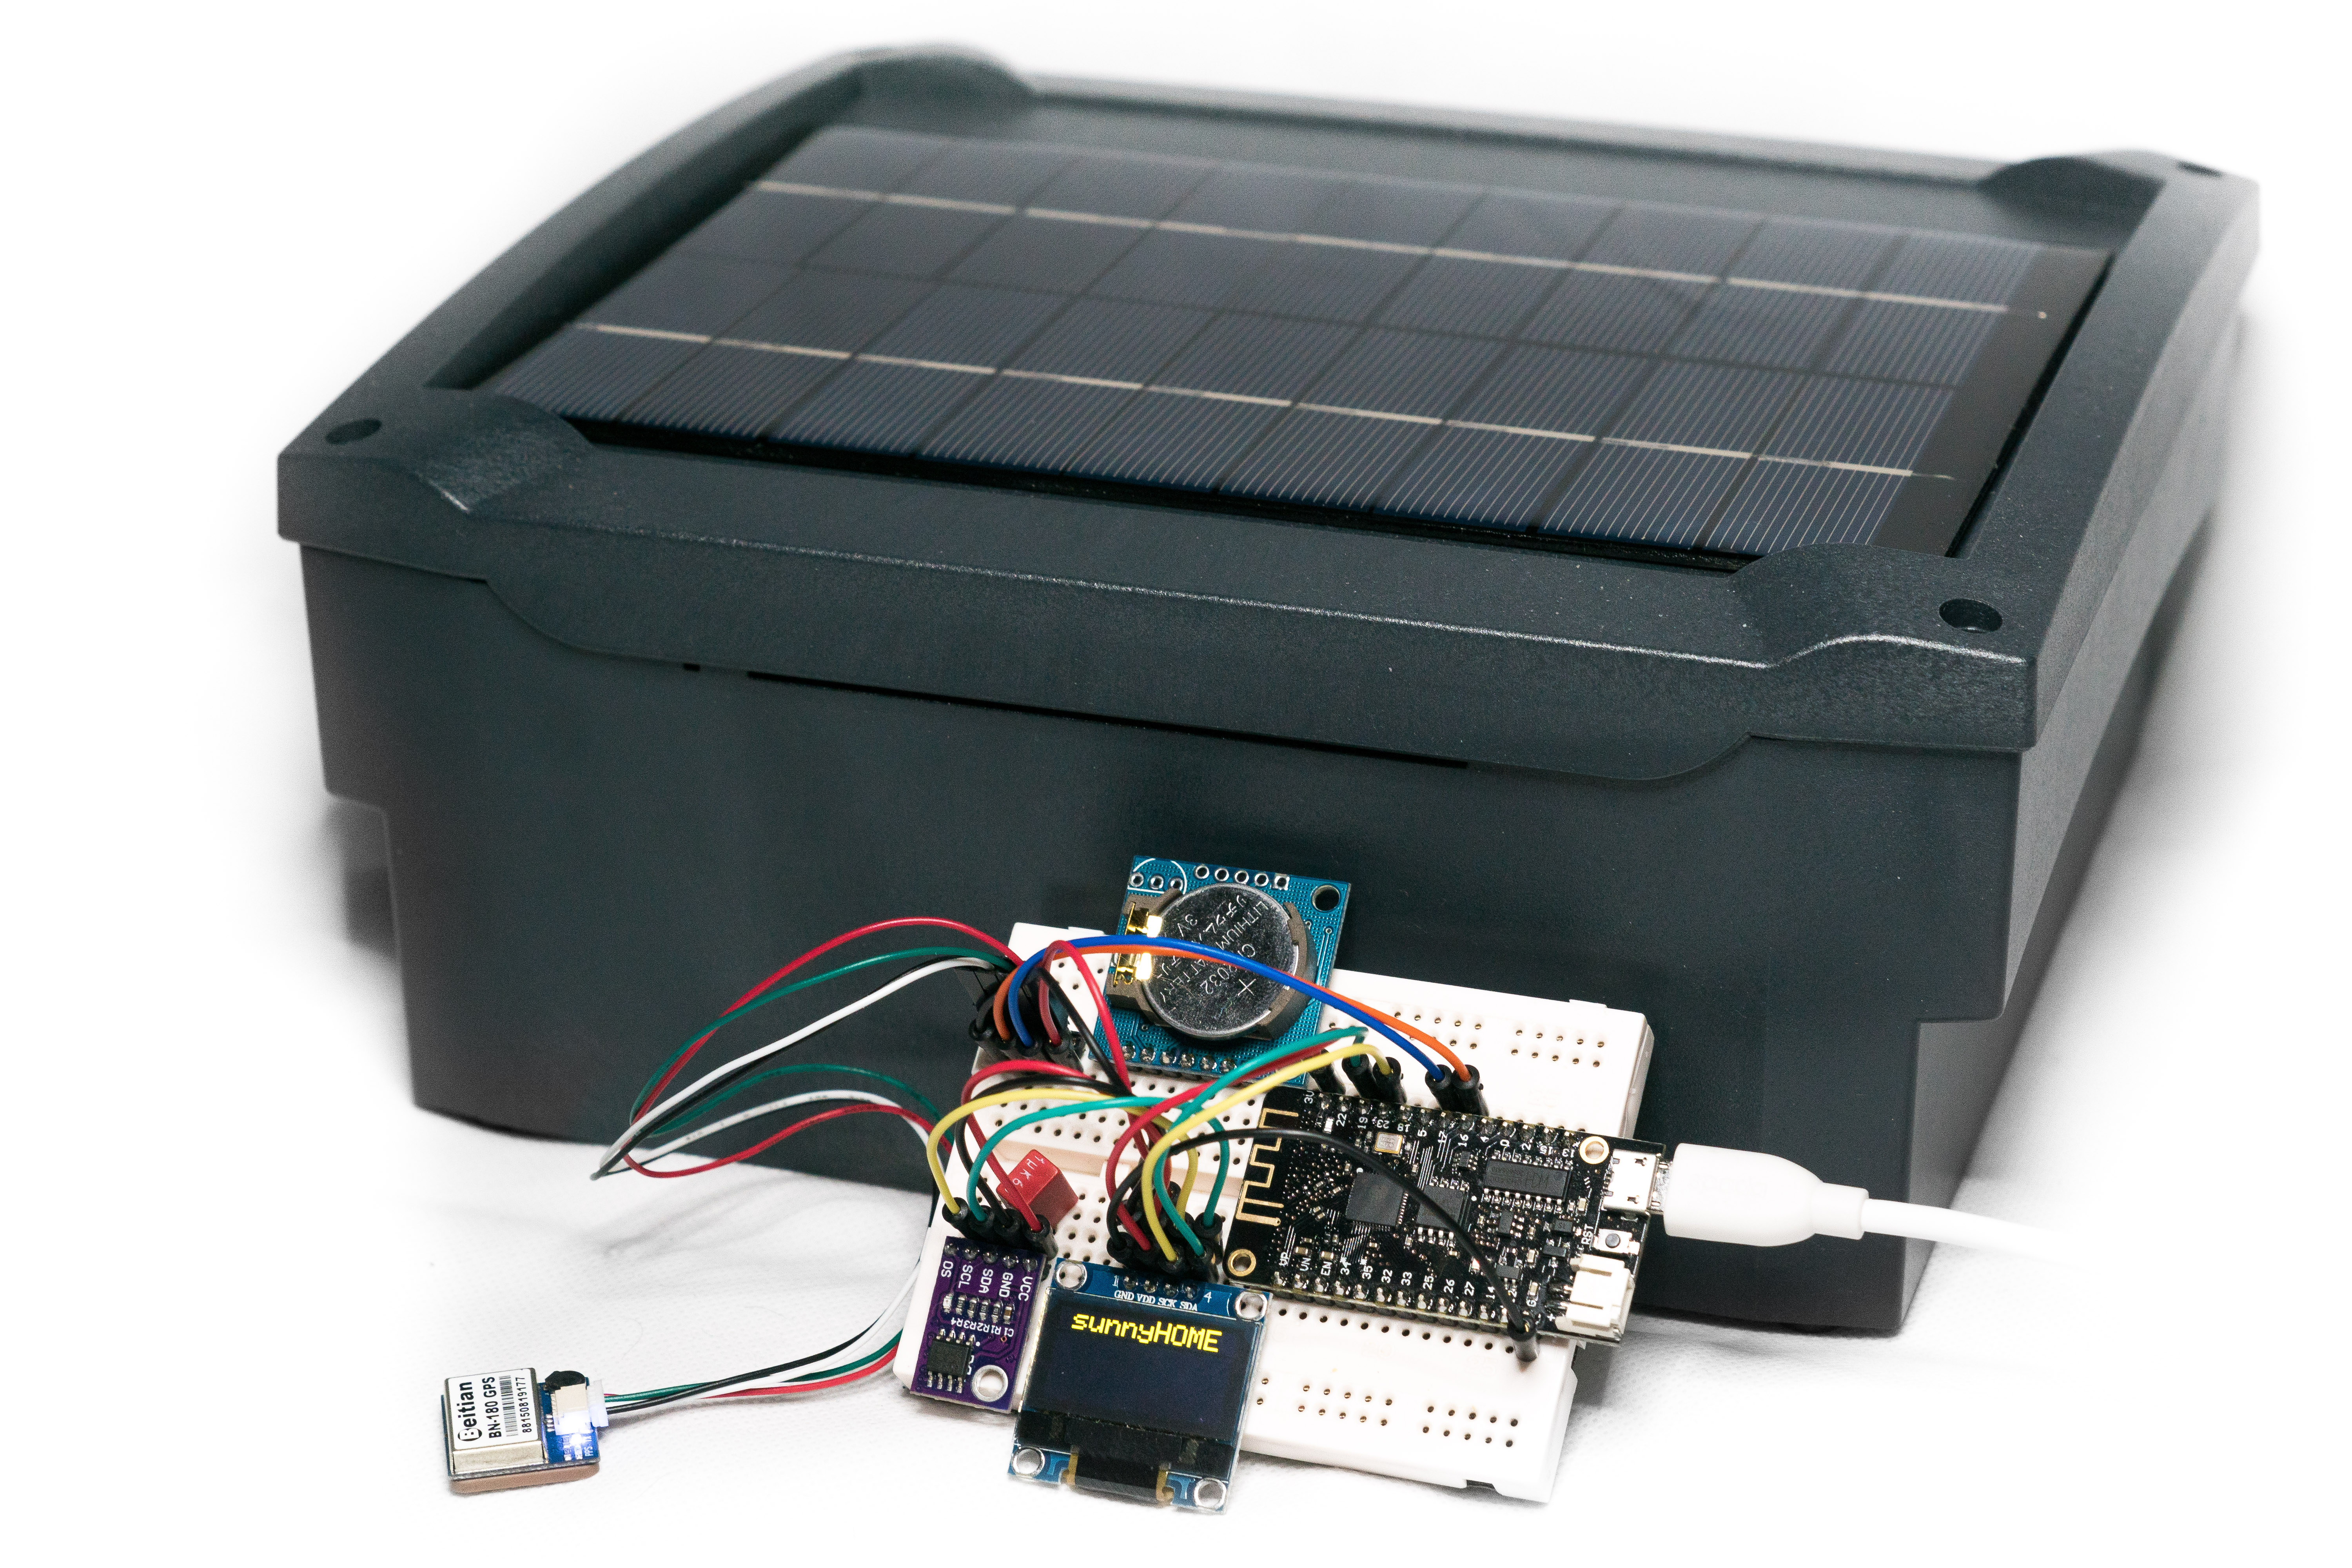
\includegraphics[width=0.7\textwidth]{./media/images/sunnyHOME.png}
        \caption{sunnyHOME-Logo}
        \label{fig:Logo}
    \end{figure}
    
    sunnyHOME ist ein Gerät, welches Wetterdaten sammelt und kabellos an einen Empfänger weiter sendet. 
    
    Es können verschiedene Sensoren, wie zum Beispiel Niederschlags- und UV-Sensoren verwendet werden. Die Daten der Sensoren werden dann über einen Mikrocontroller eingelesen und an einen Web-Server gesendet. Dieser wertet die Daten aus, die dann über eine Website oder eine App visualisiert werden. Somit kann man von überall auf der Welt nachschauen, ob die Blumen im Garten genug Wasser bekommen oder nicht.  

    
    

\pagebreak

%	--------------------------------------------------------
% 	Section 2:  Organisation
%	--------------------------------------------------------
\section{Organisation}
Das Projekt ``sunnyHOME'' wurde mit Hilfe von verschiedenen Tools organisiert. Die grundlegendsten sind in den folgenden Seiten beschrieben.
%\begin{description}

    \subsection{Microsoft To-Do}

        \begin{figure}[H]
            \centering
            \includegraphics[width=1\textwidth]{./media/images/TO-DO.png}
            \caption{Microsoft To-Do Screenshot}
            \label{fig:ToDo}
        \end{figure}
        
        \ \\ Microsoft To-Do ist eine übliche To-Do-Listen Applikation. Sie ist für Windows, Android sowie iOS verfügbar. Man kann zwischen Aufgabenbereichen trennen, und den einzelnen Aufgaben Termine zuweisen. Erstellte Termine werden über das Microsoft-Konto synchronisiert, und um einen guten Überblick über die kommende Agenda zu haben, im Kalender angezeigt.

\pagebreak
        
    \subsection{Excel}\label{ref:Protokoll}
    
        \ \\ Mit Hilfe von Microsoft Excel, sind die Arbeitszeiten und die durchgeführten Arbeitsschritte protokolliert worden. Man kann angeben, zu wie viel Prozent ein Arbeitsschritt fertiggestellt worden ist und ebenfalls Beschreibungen hinzufügen, was genau durchgeführt worden ist, wo sich Probleme ergeben haben, und was das nächste Mal gemacht werden sollte.
    
        \begin{figure}[H]
            \centering
            \includegraphics[width=1\textwidth]{./media/images/Excel.jpg}
            \caption{Protokoll Screenshot}
            \label{fig:Protokoll}
        \end{figure}
        
        Gerade bei größeren Projekten ist es sehr wichtig, Arbeitsschritte aus der Vergangenheit zurückverfolgen zu können. Sobald eine Woche nicht mehr gearbeitet wird, sind oft wichtige Ziele oder nicht vervollständigte Schritte vergessen. 
        
\pagebreak
        
        \subsubsection{Zeitplan}
        \begin{figure}[H]
            \centering
            \includegraphics[width=1\textwidth]{./media/images/Zeitplan.jpg}
            \caption{Zeitplan Screenshot}
            \label{fig:Zeitplan}
        \end{figure}
        
        Der in Excel erstellte Zeitplan ist quasi das Gegenstück zum Protokoll (siehe: \ref{ref:Protokoll}). Er visualisiert einem die kommenden Termine, und welche Arbeitsschritte in welcher Woche zu erledigen sind. Der Plan ist in Kalenderwochen strukturiert, wobei nur Arbeitstage gezählt werden. Außerdem werden einem zu beachtende Termine, Feiertage und Events neben den einzelnen Wochen angezeigt.
        
\pagebreak
        
        \subsubsection{Objektstrukturplan}\label{ref:Objektstrukt}
        
        Ebenfalls in Excel wurde ein Objektstrukturplan erstellt. Dieser orientiert sich an Projektergebnissen. Diese Projektergebnisse werden dann in Teilergebnisse aufgeteilt und hierarchisch untereinander gegliedert. 
        
        \begin{figure}[H]
            \centering
            \includegraphics[width=1\textwidth]{./media/images/Objektstrukturplan.jpg}
            \caption{Objektstrukturplan Screenshot}
            \label{fig:Objektstrukt}
        \end{figure}
        
        Vervollständigt wird der Objektstrukturplan durch einen Projektstrukturplan. (siehe \ref{ref:Projektstrukt})
        \begin{flushright}
            \cite{bib:Strukturpl}
        \end{flushright}
        
\pagebreak
        
        \subsubsection{Projektstrukturplan}\label{ref:Projektstrukt}
        
        Ein Projektstrukturplan orientiert sich hingegen einem Objektstrukturplan (siehe: \ref{ref:Objektstrukt}) nicht am Ergebnis, sondern an den Projektphasen. Es ist direkt bemerkbar, dass dieser detaillierter ist als der Objektstrukturplan. 
        
        \begin{figure}[H]
            \centering
            \includegraphics[width=1\textwidth]{./media/images/Projektstrukturplan.jpg}
            \caption{Projektstrukturplan Screenshot}
            \label{fig:Projektstrukt}
        \end{figure}
        
        
        Die Projektphasen werden von links nach rechts ihrer Durchführungsreihenfolge angeordnet. Lediglich das Projektmanagement bleibt immer links (siehe \ref{fig:Projektstrukt}: 1), da es von Anfang bis Ende des Projektes gemacht wird. Schlussendlich endet jede Arbeitsphase mit einem Meilenstein, der das Ende der Phase kennzeichnet. 
        
        \begin{flushright}
            \cite{bib:Strukturpl}
        \end{flushright}
        
        
        
\pagebreak

    \subsection{GitHub}\label{ref:GitHub}
        \ \\ Ein großer Teil des Projektmanagements ist über GitHub gelaufen. Mit Hilfe von GitHub können andere Menschen einen kompletten Überblick über das Projekt erhalten. Dafür gibt es eine Main-Page, über welche man das Datei-Verzeichnis ansehen und eine Zusammenfassung des Projektes lesen kann. Quellcodes sind für jeden zugänglich, und sogar vergangene Veränderungen an diesen sind anschaubar. Zudem ist es möglich, ein projekteigenes Wiki zu erstellen. GitHub wurde in diesem Projekt aber hauptsächlich wegen der Online-Synchronisierung verwendet. Um die Synchronisierung leichter zu gestalten, gibt es eine Desktopanwendung, welche Veränderungen hochlädt und neuste Updates herunterlädt. Dadurch lässt es sich von jedem beliebigen PC, am Projekt weiterarbeiten. 
        
        \begin{figure}[H]
            \centering
            \includegraphics[width=0.8\textwidth]{./media/images/GitHub.jpg}
            \caption{GitHub Screenshot}
            \label{fig:GitHub}
        \end{figure}
        
\pagebreak
        
    \subsection{Microsoft Project} \label{ref:MSProject}
    
        \begin{figure}[H]
            \centering
            \includegraphics[width=1\textwidth]{./media/images/GANTT.jpg}
            \caption{Mit Microsoft Project erstelltes GANTT-Diagramm}
            \label{fig:GANTT}
        \end{figure}
        
        \ \\ Mit Microsoft Project lassen sich spielend leicht, komplexe GANTT-Diagramme erstellen. Das Diagramm macht es dann möglich, dem Betrachter einen guten Rundumblick über das gegebene Projekt zu bieten. Vor allem für Außenstehende, welche sich über das Projekt und dessen Fortschritt informieren wollen, eignet es sich hervorragend. Man sieht, wann welche Arbeitsschritte durchgeführt wurden, was zurzeit das Thema ist, und welcher Arbeitsschritt der Zukunft, zu welchem Zeitpunkt ansteht. Die angegebenen Arbeitsschritte sind hierbei die selben, welche auch im Projektstrukturplan zu finden sind (siehe \ref{ref:Projektstrukt}).
%\end{description}

\pagebreak

%	--------------------------------------------------------
% 	Section 3:  Zielsetzung
%	--------------------------------------------------------
\section{Zielsetzung}
    Es soll eine Hardware entwickelt werden, die verschiedene Wetterdaten vor Ort sammelt, und über einen Web-Server von überall abgreifbar macht. Ein weiteres Ziel ist es Mithilfe von Website und App Daten übersichtlich zu visualisieren.
    
    \underline{\textbf{Die wichtigsten 5 Meilensteine: }}
    \begin{itemize}
        \item Konzept fertig
        \item Hardware funktioniert
        \item Software funktioniert
        \item Datenübertragung funktioniert 
        \item Diplomarbeit verfasst 
    \end{itemize}
    
    \subsection{Prioritäten}
    Zum einen sollte die Wetterstation sich selbst mit Energie versorgen können. Dann sollte sie modular sein, damit Hobby-Bastler leicht zwischen Funktionalitäten wechseln können. Aus diesem Grund ist das Projekt auch Open-Source (siehe: \ref{ref:GitHub}). Es soll eine grafische Benutzeroberfläche entstehen, von der aus man alles gut im Blick hat. Die Box soll dann zusätzlich über GPS lokalisiert werden können.
    Die folgenden Meilensteine sind nach Priorität sortiert.
    
    \begin{enumerate}
        \item Ein Energie-effizientes System welches Unabhängig von einer Stromversorgung ist
        \item Ein System zur Übertragung der Daten welches Energie-effizient ist
        \item Eine Hardware die multifunktional mit verschiedenen Sensoren kompatibel ist
        \item Ein einfaches modulares System, um beliebige Sensoren anzubringen 
        \item Energie-effiziente Sensoren
    \end{enumerate}
 	% Nur zur Info

%	--------------------------------------------------------
% 	KAPITEL 2: Grundlagen
%	-------------------------------------------------------	
% !TEX root = ../Vorlage_DA.tex
%	########################################################
% 				Aufgabenstellung/Pflichtenheft
%	########################################################


%	--------------------------------------------------------
% 	Überschrift, Inhaltsverzeichnis
%	--------------------------------------------------------
\chapter{Grundlagen}

%	--------------------------------------------------------
% 	Was ist IoT?
%	--------------------------------------------------------
    \section{Was ist IoT?}\label{ref:IoT}
        IoT ist heutzutage nicht weg zu denken. Deswegen bedarf der Begriff an dieser Stelle einer Erklärung. 
        Das „Internet of Things“ (IoT oder auch zu Deutsch „Internet der Dinge“) verbindet Physisches und Virtuelles miteinander und publiziert dann im Endeffekt gesammelte Informationen. So sollen zum Beispiel immer kleiner werdende Computer, Menschen bei Tätigkeiten unterstützen. Diese werden sogar in Kleidung eingearbeitet, damit eingebaute Sensoren Daten sammeln können. Die Daten werden im Endschritt über das Internet publiziert, worüber man diese dann von überall auf der Welt einsehen kann. 
        
        \begin{figure}[H]
            \centering
            \includegraphics[width=0.5\textwidth]{./media/images/IoT.jpg}
            \caption{IoT Imagebild \cite{bib:betanews}}
            \label{fig:IoT}
        \end{figure}
        
        Eine weitere Veränderung, welche mit IoT kommt ist, dass veraltete Techniken von der Idee her komplett neu überarbeitet werden. Wie zum Beispiel bei einer normalen Klingel. Früher konnte sie nur eins: klingeln. Heute verfügen Klingeln über Bewegungssensoren, Kameras und Mikrofone, um einem über alles Bescheid zu geben was vor der Tür passiert.  
        
        IoT findet sich nicht nur im privaten Gebrauch. Ein Begriff, welcher große Gemeinsamkeiten aufweist wäre „Industrie 4.0“ (oder auch Industrial Internet). Beide Gebiete haben das Ziel, Geräte und Maschinen zu vernetzen.

\pagebreak


%	--------------------------------------------------------
% 	Energieeffiziente Systeme
%	--------------------------------------------------------
\section{Energieeffiziente Systeme}
Energy-Harvesting ist in dieser Diplomarbeit ebenfalls ein Thema, da eine Energie-autarke Stromversorgung für die Wetterstation nötig ist. Aber dann stellt sich die Frage: Was ist Energy-Harvesting eigentlich?

\begin{figure}[H]
    \centering
    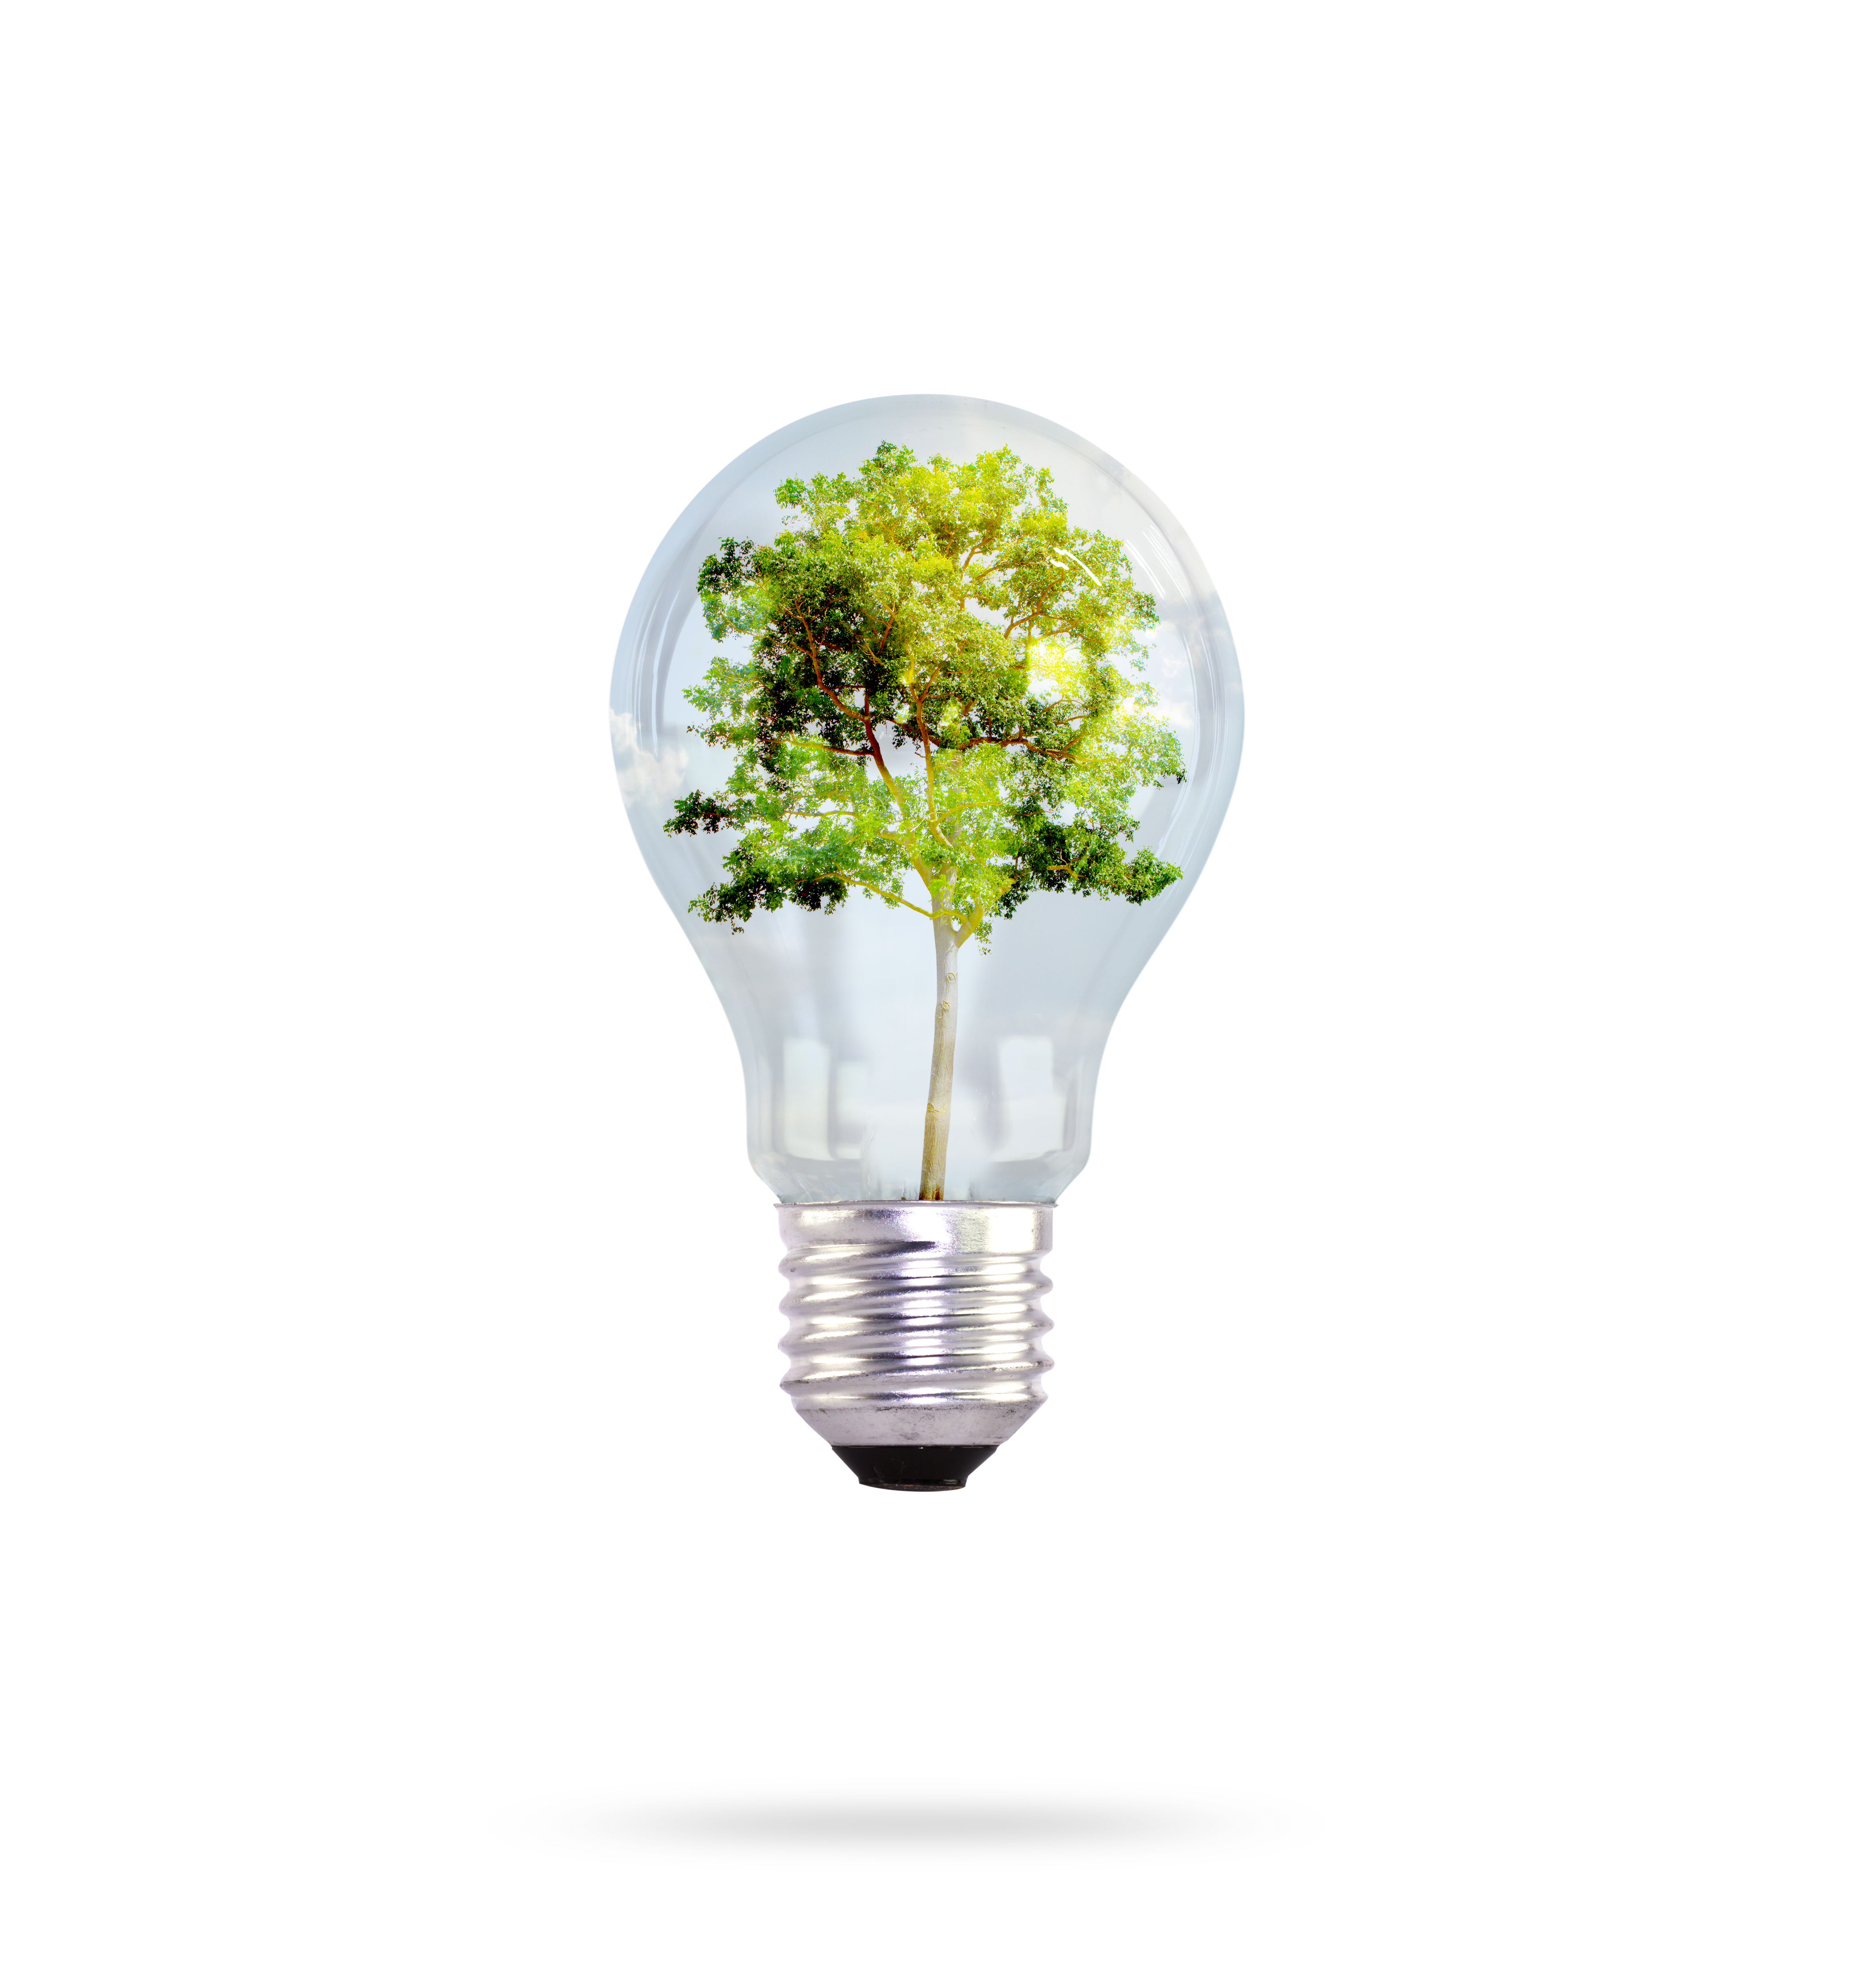
\includegraphics[width=0.7\textwidth]{./media/images/greenenergy.jpg}
    \caption{Green Energy Imagebild \cite{bib:genergy}}
    \label{fig:genergy}
\end{figure}

Beim Energy-Harvesting geht es grundsätzlich darum, die verlorene Energie einer Funktionalität zumindest teilweise wiederzuverwerten. Es ist ja zurzeit so, dass wir Energiequellen nicht vollkommen effektiv nutzen. Man nehme zum Beispiel Kohlekraftwerke: Diese haben heutzutage einen Wirkungsgrad von 40\% \cite{bib:kohle}. 

Energy-Harvesting ist im speziellen jedoch für kleinere Projekte mit niedrigem Stromverbrauch gedacht. Wie zum Beispiel für eine kleine Wetterstation. Andere Anwendungsbeispiele wären zum Beispiel Uhren, welche durch Erschütterung ihre Energie beziehen oder Sensoren, welche dank Wärmeeinstrahlung funktionieren.
 	% Nur zur Info

%	--------------------------------------------------------
% 	KAPITEL 3: Konzept (Aufgabenstellung / Pflichtenheft)
%	--------------------------------------------------------		
% !TEX root = ../Vorlage_DA.tex
%	########################################################
% 				Aufgabenstellung/Pflichtenheft
%	########################################################


%	--------------------------------------------------------
% 	Überschrift, Inhaltsverzeichnis
%	--------------------------------------------------------
\chapter{Konzept}

%	--------------------------------------------------------
% 	Grundlegende Idee
%	--------------------------------------------------------
    \section{Grundlegende Idee}\label{ref:Konzept}
    
        sunnyHOME sollte eine Wetterstation werden, welche für jeden Hobby-Elektroniker leicht zu bedienen und zu konfigurieren ist. Man sollte sie einfach in den Wald stellen können, ohne sich jegliche Sorgen um Stromversorgung machen zu müssen. Das heißt sie sollte Energie-autark werden. 
        
        \begin{figure}[H]
            \centering
            \includegraphics[width=0.5\textwidth]{./media/images/Schema.png}
            \caption{Aufbau der Wetterstation.\cite{bib:HugoGomes}}
            \label{fig:Aufbau}
        \end{figure}
        
        Ebenfalls sollte eine Funkverbindung implementiert werden. Dies wäre nötig, um eine Kommunikation über mehrere Kilometer gewährleisten zu können. 
        
        In einem weiteren Schritt sollte eine intuitive Website und App programmiert werden. Über diese sollte man dann die empfangenen Sensordaten auslesen, und den Standort der Wetterstation abrufen können. 
        
        
%	--------------------------------------------------------
% 	Kommunikation
%	--------------------------------------------------------
    \section{Kommunikation}
    
         Ein ESP32 (siehe: \ref{ref:ESP32}) hat standardmäßig WLAN und Bluetooth verbaut. Ein Ziel des Projektes war jedoch, die Positionierung der Wetterstation, weit weg von jeglichen WLAN-Netzen und Bluetooth-Receivern zu positionieren. Um dies zu verwirklichen war zuerst ein Funk-Modul vorgesehen. 
         Im späteren Laufe des Projektes, wurde die Kommunikation über WLAN vorgezogen, da diese keine zusätzliche Hardware für einen MQTT-Broker braucht, und Zeit aufgeholt werden musste.
        
\pagebreak
        
%	--------------------------------------------------------
% 	Energie-Management
%	--------------------------------------------------------
    \section{Energie-Management}
    
         Für die Energie-Versorgung ist eine 9V-Solarzelle beschaffen worden. Diese wurde anderen Solarzellen vorgezogen, weil sei eine bessere „Low-Light Performance“ bietet. Da sie eine höhere Spannung liefert, können kleinere Ströme wahrgenommen werden, welche dann über ein Energy-Harvesting Modul den Akku speisen.
        
        \begin{figure}[H]
            \centering
            \includegraphics[width=0.3\textwidth]{./media/images/SolarPanel.jpg}
            \caption{9V Solarzelle \cite{bib:SolarPanel}}
            \label{fig:SolarPanel}
        \end{figure}
        
        Energy-Harvesting Module können wie Kondensatoren verstanden werden. Sie werden mit niedrigen Strömen aufgeladen, und wenn sie sich dann aufgeladen haben, wird der ganze Strom mit einen Schub in den Akku gespeist. Nötig ist das, da Akkus keine zu niedrigen Ströme aufnehmen können. 
        
        Um zusätzlich an Energie zu sparen, gibt es beim ESP32 verschiedene \textbf{„Power-Modes“}: 
        
        \begin{itemize}
            \item \textbf{Active Mode: }        Der Chip ist voll funktionstüchtig. Er kann Empfangen, Versenden und Zuhören
            \item \textbf{Modem-Sleep Mode: }	Der CPU ist betriebsbereit und der Takt lässt sich konfigurieren. Funkverbindungen sind ausgeschalten
            \item \textbf{Light-Sleep Mode: }	Der CPU ist pausiert. Der RTC-Speicher und die RTC-Peripherien (RTC ... Real-Time Clock), sowie der ULP Co-Prozessor (ULP ... Ultra-Low-Power) sind am Laufen. Verschiedene Wake-Up Events können das Aufwachen des Chips verursachen. 
            \item\label{ref:DeepSleep} \textbf{Deep-Sleep Mode: }    Nur der RTC-Speicher und die RTC-Peripherien sind eingeschalten. Verbindungsdaten sind im RTC-Speicher gespeichert. ULP Co-Prozessor ist funktionsbereit. 
            \item \textbf{Hibernation Mode: }   Der interne 8MHz Oszillator und der ULP Co-Prozessor sind ausgeschalten. Nur der RTC-Timer am langsamen Tackt und einige RTC GPIOs sind aktiv. Der RTC-Timer oder die RTC-GPIOs können den Chip aus dem Hibernation Mode aufwecken. 
        \end{itemize}
        \begin{flushright}
            \cite{bib:esp32datasheet}
        \end{flushright}
        Im Programm wurde der Deep-Sleep Mode gewählt. Es kann ein Intervall eingestellt werden, in dem der ESP immer hochfährt, die Daten sendet, und dann wieder in den Schlaf-Modus zurückkehrt. 
        
\pagebreak

         
%	--------------------------------------------------------
% 	Visualisierung
%	--------------------------------------------------------
    \section{Visualisierung}
    
         Wie bereits in \ref{ref:Konzept} erwähnt, sollte eine App und eine Website realisiert werden. Hauptanliegen dieser Applikationen waren: 
         
         \begin{itemize}
            \item   eine umfassende Übersicht über gemessene Sensordaten
            \item   das Tracken der Wetterstation
            \item   eine intuitive, benutzerfreundliche Oberfläche
            \item   die Möglichkeit Einstellungen des ESP zu verwalten
        \end{itemize}
        
        Um das Pensum des Projektes zu kürzen, musste auf die Entwicklung von eigenen Applikationen verzichtet werden. Dafür wurde ein online MQTT-Broker implementiert, welcher es möglich macht, alle obigen Punkte zu realisieren (siehe: \ref{ref:Ubidots}).
        
         
%	--------------------------------------------------------
% 	Funktionsablauf
%	--------------------------------------------------------
    \section{Funktionsablauf} \label{ref:FnktAb}
    
        Für den Funktionsablauf des Programms wurde eine Struktur festgelegt. In der folgenden Abbildung \ref{fig:FnktAb} sieht man, nach welcher Reihenfolge die Teilaufgaben des Programms geordnet sind. 
    
         \begin{figure}[H]
            \centering
            \includegraphics[width=1\textwidth]{./media/images/FnktAb.jpg}
            \caption{Illustration zum Funktionsablauf}
            \label{fig:FnktAb}
        \end{figure}
        
        Sobald der Controller aus dem Deep-Sleep Mode (siehe: \ref{ref:DeepSleep}) aufwacht, soll versucht werden, eine Verbindung zum Internet und zum MQTT-Broker aufzubauen. Ist dies geschehen, wird auf GPS-Daten Empfang gewartet. Sobald sie dann empfangen werden, wird die RTC mit der GPS-Zeit synchronisiert. Danach erfolgen die Sensor-Messungen, welche im nächsten Schritt, zusammen mit den GPS-Daten, an den MQTT-Broker versendet werden sollen. Ist die Routine zu Ende, wird der Deep-Sleep Modus wieder gestartet, und der Timer gestellt, nachdem der Controller wieder aufwachen soll.  
         


%	--------------------------------------------------------
% 	KAPITEL 4: Umsetzung 
%	--------------------------------------------------------	
% !TEX root = ../Vorlage_DA.tex

%	########################################################
% 				Entwurf
%	########################################################


%	--------------------------------------------------------
% 	Überschrift, Inhaltsverzeichnis
%	--------------------------------------------------------
\chapter{Umsetzung}

%	--------------------------------------------------------
% 	Hardware
%	--------------------------------------------------------
\section{Hardware}

\subsection{LM75A}\label{ref:LM75A}

    Der LM75A ist ein Temperatursensor, welcher via I$^2$C kommuniziert. In der folgenden Abbildung \ref{fig:LM75A} ist er zu sehen.

    \begin{figure}[H]
        \centering
        \includegraphics[width=0.5\textwidth]{./media/images/lm.jpg}
        \caption{LM75A\cite{bib:LM75A}}
        \label{fig:LM75A}
    \end{figure}

    Die Messung der Temperatur ist eine der grundlegendsten Funktionen, welche eine Wetterstation können soll. Zusätzlich ist der LM75A mit einem Durchmesser von 23mm sehr klein und billig in der Anschaffung. 
    
    Um Störgrößen zu vermeiden, wurde ein kleiner Kondensator mit 1 $\mu F$, zwischen Versorgung und Ground verbaut. 

\pagebreak

\subsection{ESP8266}\label{ref:ESP8266}

    \begin{figure}[H]
        \centering
        \includegraphics[width=0.3\textwidth]{./media/images/ESP8266.jpg}
        \caption{ESP8266\cite{bib:ESP8266}}
        \label{fig:ESP8266}
    \end{figure}

    Angefangen wurde das Projekt mit dem ESP8266. Dieser ist ein Mikrocontroller, welcher unter Arduino spielend leicht programmierbar ist. Positive Aspekte dessen sind, dass es viele stabile Bibliotheken gibt, welche von vielen Nutzern verwendet werden. Nur ist der ESP8266 unbrauchbar geworden, als es um energiesparendere Wege ging. So musste dann ein neuer Mikrocontroller verwendet werden (siehe \ref{ref:ESP32}).

\subsection{ESP32} \label{ref:ESP32}

    Der ESP32 ist ein Mikrocontroller aus dem Hause Espressif. Er eignet sich ideal für IoT-Projekte (siehe: \ref{ref:IoT}), da er WLAN und Bluetooth an Bord hat. Außerdem besitzt er einen Dual-Core Prozessor, welcher für erhöhte Energie-Effizienz ausgelegt ist. 
    
    \begin{flushright}
            \cite{bib:ESP32Erw}
    \end{flushright}

    \begin{figure}[H]
        \centering
        \includegraphics[width=0.3\textwidth]{./media/images/ESP32.jpeg}
        \caption{ESP32 \cite{bib:ESP32}}
        \label{fig:ESP32}
    \end{figure}

    Nachdem der ESP8266 (siehe: \ref{ref:ESP8266}) nicht genügend Energie-effizient war,  ist der ESP32 als neuer Controller ausgewählt worden. Dieser hat nämlich einen Deep-Sleep Modus \ref{ref:DeepSleep} integriert. Probleme hat es mit dem ESP32 jedoch auch gegeben. Viele Bibliotheken, welche es für den ESP32 gibt, sind nicht zuverlässig. Oft musste bei diesen für das eigene Projekt nachgebessert werden. 
    
\pagebreak

\subsection{GPS-Modul}\label{ref:Beitian}

    Der u-blox M8030-KT ist ein GPS-Empfänger, welcher über Serielle Schnittstelle angesprochen wird. In diesem Projekt ist er in einem Modul von Beitian verbaut (siehe Abbildung \ref{fig:Beitian}). Über HardwareSerial.h wird der empfangene Datenstrom des GPS-Empfängers ausgelesen. Dieser Datenstrom kann dann mithilfe der Bibliothek „TinyGPS++.h“ verwertet werden.
    
    \begin{figure}[H]
        \centering
        \includegraphics[width=0.4\textwidth]{./media/images/GPS.jpg}
        \caption{Beitian BN-180 im Vergleich zu einer Münze \cite{bib:Beitian}}
        \label{fig:Beitian}
    \end{figure}
    
\subsection{Real-Time Clock}\label{ref:RTC}

    Die Echtzeituhr DS1307 ist ein Modul zum Zählen der Zeit. Sie hat einen integrierten Speicher und ist sehr Energie-effizient. Wenn die Echtzeituhr nicht über den Controller versorgt wird, gibt es die Möglichkeit, eine Batterie zu platzieren. Die Kommunikation mit dem Controller verläuft über I$^2$C.  

    \begin{figure}[H]
        \centering
        \includegraphics[width=0.3\textwidth]{./media/images/DS1307.jpg}
        \caption{DS1307 Real-Time Clock \cite{bib:DS1307}}
        \label{fig:DS1307}
    \end{figure}
    
    Der ESP32 hat eigentlich bereits eine Real-Time Clock verbaut. Nur ist diese nicht präzise genug und verfälscht die Zeit auf lange Sicht. Deswegen wurde sich für den DS1307 entschieden. 

\pagebreak

%	--------------------------------------------------------
% 	Realisierte Lösungen
%	--------------------------------------------------------
\section{Software}

    \subsection{Atom Editor}\label{ref:Atom}
    
        Atom ist ein moderner Texteditor, welcher sich durch verschiedenste Pakete, Bibliotheken und Designs erweitern und modifizieren lässt. Da Atom ein Produkt von GitHub ist, funktioniert die Anbindung daran einwandfrei. Außerdem gibt es eine Menge an nützlichen Tools, wie zum Beispiel die „smarte Autokorrektur“.  
        
        \begin{flushright}
            \cite{bib:AtomTipps}
        \end{flushright}
        
        In der folgenden Abbildung (\ref{fig:Atom}) sieht man einen Screenshot des Atom-Editors. 
    
        \begin{figure}[H]
            \centering
            \includegraphics[width=1\textwidth]{./media/images/AtomScreenshot.jpg}
            \caption{Atom Screenshot\cite{bib:Atom}}
            \label{fig:Atom}
        \end{figure}
        
        Gewählt wurde der Atom-Editor, da man ihn auf den meisten Platformen installieren kann und die Installation ebenfalls keine große Hürde ist. Und wie bereits erwähnt wurde, sind die Funktionalitäten dieses Editors sehr praktisch. Um jedoch einen ESP32 programmieren zu können reicht ein gewöhnlicher Texteditor nicht aus. Aus diesem Grund musste das PlatformIO-Paket installiert werden (siehe \ref{ref:PlatformIO}). 
        
    
\pagebreak

    \subsection{PlatformIO}\label{ref:PlatformIO}
    
    PlatformIO ist eine IDE\footnote{Wikipedia-Eintrag: https://de.wikipedia.org/wiki/Integrierte\_Entwicklungsumgebung, 06. April 2019}, welche im speziellen für das Programmieren von Mikrocontrollern gedacht ist. Es lassen sich die geschriebenen Codes auf Fehler überprüfen, man hat die Möglichkeit die geschriebenen Programme mit Kabel oder kabellos auf den Controller zu laden, und ein Serieller Monitor, über welchen man Nachrichten des Mikrocontrollers empfangen kann, ist ebenfalls verbaut.
    
    \begin{figure}[H]
        \centering
        \includegraphics[width=1\textwidth]{./media/images/PlatformIO.jpg}
        \caption{PlatformIO Screenshot\cite{bib:PlatformIO}}
        \label{fig:PlatformIO}
    \end{figure}
    
    Entschlossen wurde sich für diese IDE, da diese eine Lösung für die Programmierung mit Atom (siehe: \ref{ref:Atom}) gewesen ist.
    
    
    
\pagebreak

\subsection{Ubidots \cite{bib:ubidots}}\label{ref:Ubidots}
    
    Ubidots ist ein MQTT-Broker, welcher wie ein Cloud-Service funktioniert. Mit Hilfe von Ubidots lassen sich die Daten eines Mikrocontrollers spielend leicht im Internet publizieren und visualisieren. Man kann sich beispielsweise Statistiken über Temperaturunterschiede der letzten Wochen anzeigen lassen, oder natürlich ebenfalls auf aktuell aufgenommene Daten wie GPS-Standort zugreifen. 
    
    \begin{figure}[H]
        \centering
        \includegraphics[width=1\textwidth]{./media/images/ubidotsSC.jpg}
        \caption{Ubidots-Dashboard Screenshot\cite{bib:ubidots}}
        \label{fig:ubidots}
    \end{figure}
    
    Zu Beginn des Matura-Projektes, ist noch das Erstellen einer eigenen Website und einer eigenen App geplant gewesen. Da das Projekt schlussendlich doch alleine durchgeführt wurde, musste eine einfachere Lösung gefunden werden. So wurde dann Ubidots als Darstellungs-Plattform gewählt. 

\pagebreak

\section{Bibliotheken}
    \subsection{HardwareSerial.h}
    
        Die „HardwareSerial-Bibliothek“ behandelt die Hardware-Schnittstellen (UART) des ESP32. Grundsätzlich sind am Mikrocontroller drei Schnittstellen verbaut. Die standardmäßige Pinbelegung der Schnittstellen kann jedoch problematisch werden, da dieselben Pins zum Beispiel die Ansteuerung des internen Flashspeichers oder Reseteingänge belegen. Dafür bietet der ESP32 aber eine einfache Lösung: Mit Hilfe der HardwareSerial Bibliothek lassen sich die Hardware-Schnittstellen mit beinahe jedem IO-Pin verbinden.
        \begin{flushright}
            \cite{bib:HWSerial}
        \end{flushright}
        
        In Listing \ref{code:HWSerial} wird die Implementierung der seriellen Schnittstelle des GPS-Moduls gezeigt. Über diese werden im eingeschalteten Modus dauerhaft GPS-Daten an den Controller geliefert. 
        \begin{lstlisting}[
            language=c,
            caption={HardwareSerial Initialisierung },
            label=code:HWSerial
        ]
////                GPS-Reseiver                    ////
HardwareSerial gps(2); // (2) weil UART2

void setup() {
  // Datenrate: 9600 Bit/s, Rx-Pin: 16, Tx-Pin: 17
  gps.begin(9600, SERIAL_8N1, 16, 17); 
}
        \end{lstlisting}
    
    \subsection{Wire.h}
        Die „Wire-Bibliothek“ erlaubt es einem, via I$^2$C zu kommunizieren. Sie hat eine ähnliche Funktionalität wie die „HardwareSerial-Bibliothek“. In dem man die gewünschten Pins in „Wire.begin()“ einfügt, lässt sich die I$^2$C-Kommunikation einstellen. Wenn nichts eingefügt wird, werden die Standard Pins gewählt. 
        
        Nachdem ein ESP32-Devboard während des Jahres kaputt gegangen ist, musste bei dem nächsten ESP32-Board auf die Standard Pin-Belegung verzichtet werden. Aus diesem Grund mussten, wie in Listing \ref{code:Wire} beschrieben, die Pins neu definiert werden. 
        \begin{lstlisting}[
            language=c,
            caption={I2C Konfiguration},
            label=code:Wire
        ]
#include <Wire.h>

void setup() {
  // SDA: 19, SCL: 23
  Wire.begin(19,23); 
}
        \end{lstlisting}
        
        Somit läuft die komplette I$^2$C-Kommunikation über die ausgewählten Pins. Werden jedoch Bibliotheken, welche man für I$^2$C-Bausteine eingebunden hat verwendet, muss aufgepasst werden, dass diese Pin-Belegung nicht verändert wird. 
        
\pagebreak
    
    \subsection{WiFi.h \& PubSubClient.h}
        
        Die ESP32-Bibliothek „WiFi.h“ ist für die Verbindung zum WLAN-Netz verantwortlich. Im folgenden Listing \ref{code:WiFi} ist der Code für die Verbindung zu einem WLAN-Netzwerk zu sehen. Es wird nur das einfügen des WLAN-Namen und WLAN-Passwortes benötigt.
        
        \begin{lstlisting}[
            language=c,
            caption={WLAN Konfiguration},
            label=code:WiFi
        ]
#include <WiFi.h>

void setup() {
  WiFi.begin(WIFISSID, PASSWORD); 
}
        \end{lstlisting}
        
        Um eine Verbindung zu einem MQTT-Broker herzustellen braucht es aber noch mehr. Dazu wird die Bibliothek „PubSubClient.h“(Publish-Subscribe Client) benötigt. Diese ermöglicht es einem, MQTT-Topics zu versenden. Listing \ref{code:payload} zeigt die Publikation des Temperatur-Topics.
        
        \begin{lstlisting}[
            language=c,
            caption={Erstellen der Payload und Publikation der Temperatur},
            label=code:payload
        ]
/**********   Temperatur-Publikation   ***********/
//  hier wird die ID des Ubidots-Gerätes eingetragen
sprintf(topic, "%s%s", "/v1.6/devices/", DEVICE_LABEL);
// payload wird gereinigt
sprintf(payload, "%s", ""); 
//  hier wird die ID der Ubidots-Variable eingetragen
sprintf(payload, "{\"%s\":", VARIABLE_LABEL_TEMP);
//  hier wird der String mit der Temperatur eingetragen
sprintf(payload, "%s {\"value\": %s}}", payload, str_temperature);
//  Datenpaket wird versendet
client.publish(topic, payload);
        \end{lstlisting}
        
        Das verschickte Datenpaket (die Payload) sieht folgendermaßen aus:
        \begin{center}
            \{''temperature``: \{''value``: 26.37\}\}
        \end{center}
    
    \subsection{DS1307.h}
    
        Die Bibliothek „DS1307.h“ ist für die RTC (Real-Time Clock, siehe: \ref{ref:RTC}) zuständig. Um die aktuelle Zeit einzutragen, wird die GPS-Zeit mit der RTC-Zeit periodisch synchronisiert. 
        
        In Listing \ref{code:time} ist das Eintragen der GPS-Zeit und des GPS-Datums in die Real-Time Clock zu sehen.  
        
        \begin{lstlisting}[
            language=c,
            caption={Synchronisierung der GPS-Zeit mit der RTC-Zeit},
            label=code:time
        ]
#include <DS1307.h>
RTC_DS1307 rtc;

void setup() {
  rtc.begin()
  //  TinyGPSDate &d ... GPS-Datum, TinyGPSTime &t ... GPS-Zeit
  rtc.adjust(DateTime(d.year(), d.month(), d.day(), t.hour(), t.minute(), t.second()));  
}
        \end{lstlisting}
        
    \subsection{TinyGPS++.h}
    
    Die Bibliothek „TinyGPS++.h“ ist vor allem für eine Sache zuständig: das Übersetzen des ankommenden seriellen Datenstroms des GPS-Receivers (siehe: \ref{ref:Beitian}).
    
    Es gibt jedoch auch einige nützliche Funktionen, welche die Bedienung des GPS-Receivers vereinfachen (siehe: Listing\ref{code:GPSFunct}). 
    
            \begin{lstlisting}[
            language=c,
            caption={TinyGPS++ Funktionen},
            label=code:GPSFunct
        ]
//************   GPS Functions   ************//
//  Entschlüsselt Datenstrom
static void smartDelay(unsigned long ms);
//  Gibt gewünschte Daten als Float im Seriellen Monitor aus 
static void printFloat(float val, bool valid, int len, int prec);
//  Gibt gewünschte Daten als Integer im Seriellen Monitor aus 
static void printInt(unsigned long val, bool valid, int len);
//  Gibt aktuelles Datum und Uhrzeit im Seriellen Monitor aus
static void printDateTime(TinyGPSDate &d, TinyGPSTime &t);
        \end{lstlisting}
        
        
        
        
        Die wichtigste der Funktionen ist die „smartDelay“-Funktion. Sie entschlüsselt den ankommenden seriellen GPS-Datenstrom und packt die entschlüsselten Informationen in die „TinyGPSPlus“-Variable:
        
        \begin{lstlisting}[
            language=c,
            caption={„smartDelay“-Funktion},
            label=code:smartDelay
        ]
static void smartDelay(unsigned long ms)
{
  unsigned long start = millis();
  do
  {
//  Solange ein serieller Datenstrom ankommt, 
//  soll dieser entschlüsselt werden
    while (HWSerialGPS.available())
//  gps ist eine TinyGPSPlus-Variable
      gps.encode(HWSerialGPS.read());
  } while (millis() - start < ms);
}
        \end{lstlisting}
        
        
        
        Damit die Daten über MQTT versendet werden können, müssen sie als Strings gespeichert werden. Es gibt jedoch keine Möglichkeit, die Koordinaten als Strings zu erhalten. Dazu muss die folgende Wandlung gemacht werden: 
  
        \begin{lstlisting}[
            language=c,
            caption={Float zu String Wandlung für MQTT},
            label=code:FloatString
        ]
//      1.Parameter: Breitengrad in float               
//      2.Parameter: Zahl darf 9 Stellen lang sein 
//      3.Parameter: mit maximal 6 Nachkommastellen     
//      4.Parameter: wird in folgende String gewandelt 
dtostrf(gps.location.lat(), 9, 6, str_lat);  //  für MQTT 
dtostrf(gps.location.lng(), 9, 6, str_long); //  für MQTT
        \end{lstlisting}



%	--------------------------------------------------------
% 	Bedienungsanleitung
%	--------------------------------------------------------
% !TEX root = ../Vorlage_DA.tex
%	########################################################
% 					Bedienungsanleitung
%	########################################################


%	--------------------------------------------------------
% 	Überschrift, Inhaltsverzeichnis
%	--------------------------------------------------------
\chapter{Bedienungsanleitung}


%	--------------------------------------------------------
% 	Suche eines geeigneten Standortes
%	--------------------------------------------------------
\section{Suche eines geeigneten Standortes}
    
    \begin{figure}[H]
            \centering
            \includegraphics[width=0.8\textwidth]{./media/images/wifirange.png}
            \caption{Atom Screenshot\cite{bib:WiFiBooster}}
            \label{fig:WiFiRange}
    \end{figure}
    
    Damit sunnyHOME überhaupt Daten publizieren kann, braucht die Wetterstation einen Ort mit Verbindung zu einem WLAN-Netz. Handelsübliche WLAN-Netze geben eine mögliche Reichweite von 46 Metern in Gebäuden und 92m im Freien an \cite{bib:WiFiRange}. Diese Werte sind meist jedoch sehr optimistisch. Hat man sunnyHOME im Garten stehen, sollte man mit einer Reichweite von 35-45 Metern rechnen.
    
    Ein Ort mit guter Sonneneinstrahlung ist vorteilhaft.
    
\pagebreak
    
%	--------------------------------------------------------
% 	Einstellen von Ubidots
%	--------------------------------------------------------
\section{Einstellen von Ubidots}
 
    Für das Publizieren der gesammelten Daten wird ein Ubidots-Konto benötigt (siehe: \ref{ref:Ubidots}). Das lässt sich auf ihrer Website \url{www.ubidots.com} machen. Ist man noch Student, kann man sich über \url{www.ubidots.com/education/} ein kostenloses „Education-Konto“ erstellen. 
    
    Ist das Konto erstellt worden, muss ein „Device\footnote{Anleitung „Devices“: https://help.ubidots.com/user-guides/creating-devices-in-ubidots, 07.04.2019}“ erstellt werden. Dann braucht es noch „Variables\footnote{Was sind „Variables“: https://help.ubidots.com/faqs-and-troubleshooting/what-are-variables, 07.04.2019}“ und eine „Dashboard\footnote{Anleitung zu „Dashboards“: https://help.ubidots.com/user-guides/create-dashboards-and-widgets, 07.04.19}“. Sind diese Schritte gemacht, kann das Device wie in Screenshot \ref{fig:ubiDev} aussehen. 
    
    \begin{figure}[H]
            \centering
            \includegraphics[width=0.8\textwidth]{./media/images/ubidotsDev.jpg}
            \caption{ubidots-Device Screenshot\cite{bib:ubidots}}
            \label{fig:ubiDev}
    \end{figure}
    
\pagebreak
    
%	--------------------------------------------------------
% 	Modifizierung des Codes
%	--------------------------------------------------------
\section{Modifizierung des Codes}
 
    Der letzte Schritt bei der Einrichtung von sunnyHOME, ist das modifizieren des Codes.
    
    Sobald man das Programm in einem passenden Editor (siehe: \ref{ref:Atom}) bzw. in einer passende IDE (siehe: \ref{ref:PlatformIO}) geöffnet hat, sollte die Verbindung zu einem WLAN-Netzwerk hergestellt werden. Im Quellcode befinden sich zwei globale Konstanten, in welche man den Namen seines Netzwerkes und den Schlüssel des Netzwerkes einfügt. In Listing \ref{code:LOGIN} sind diese Konstanten zu sehen. 
    
    \begin{lstlisting}[
            language=c,
            caption={Verbindung mit WLAN-Netzwerk und Ubidots},
            label=code:LOGIN
        ]
///     WLAN Konstanten
#define WIFISSID "meinInternet"         // hier WLAN-SSID eintragen
#define PASSWORD "meinGeheimesPasswort" // hier WLAN-Passworrt eintragen
///     Ubidots Konstanten
#define TOKEN "meinUbidotsToken"        // hier Ubidots-Token eintragen
    \end{lstlisting}
    
    Im nächsten Schritt gilt es die Verbindung zum Ubidots-Broker herzustellen. Wenn man sich ubidots öffnet, findet sich ein Menü-Punkt namens „API Credentials“ (siehe: \ref{fig:ubitoken}). Von dort kopiert man sich den „Default token“, welcher ebenfalls ins Programm eingefügt wird (siehe: \ref{code:LOGIN}).
      
    \begin{figure}[H]
            \centering
            \includegraphics[width=1\textwidth]{./media/images/ubitoken.jpg}
            \caption{Ubidots-token Screenshot\cite{bib:ubidots}}
            \label{fig:ubitoken}
    \end{figure}  
    
    Jetzt fehlen nur noch die Labels. Diese sind Etiketten, welche es für jede Messung, welche über MQTT übertragen werden soll gibt. Für die Labels gibt es ebenfalls globale Konstanten (siehe: \ref{code:label}). 
    
\begin{lstlisting}[
            language=c,
            caption={MQTT-Labels},
            label=code:label
        ]
///   Labels für MQTT
#define VARIABLE_LABEL_TEMP "temperature"   // Hier Temperatur-Label eintragen
#define VARIABLE_LABEL_GPS "gps"            // Hier GPS-Label eintragen
#define DEVICE_LABEL "esp32"                // Hier Device-Label eintragen
    \end{lstlisting}
    
    Wenn die eingetragenen Labels mit den in Ubidots eingetragenen API-Labels identisch sind, sollte die Übertragung der Daten per MQTT nun funktionieren. 

    
    
    
\pagebreak



%	--------------------------------------------------------
% 	Fazit und Persönliche Erfahrungen
%	--------------------------------------------------------
% !TEX root = ../Vorlage_DA.tex

%	########################################################
% 					Fazit und Persönliche Erfahrungen
%	########################################################



%	--------------------------------------------------------
% 	Überschrift, Inhaltsverzeichnis
%	--------------------------------------------------------
\chapter{Fazit und Persönliche Erfahrungen}


%	--------------------------------------------------------
% 	Fazit
%	--------------------------------------------------------
\section{Fazit}

\subsection{Zusammenfassung der Ergebnisse}
    Im Großen und Ganzen wurden die wichtigsten Themenstellungen des Projektes behandelt und fertiggestellt. Einzig die Energie-Versorgung ist nicht fertig realisiert worden.
    
    Die Software funktioniert und der Funktionsablauf des Codes (siehe: \ref{ref:FnktAb}) ist fertiggestellt. Die Verbindung zu Ubidots (siehe: \ref{ref:Ubidots} ist stabil und es lassen sich die gewünschten Messwerte im Internet betrachten. Der Mikrocontroller wechselt ebenfalls nach dem Erfüllen seiner Aufgaben in den Deep-Sleep Modus, um dadurch Energie zu sparen.  

\subsection{Mögliche Erweiterungen}
    Damit die Wetterstation wirklich fertiggestellt ist, muss die Energie-Versorgung durch die Solarzellen fertiggestellt werden. Dafür werden Energieverbrauchs-Messungen am ESP32 benötigt, dann kann man erst den Energy-Harvesting Modul bestimmen. Und in Abhängigkeit des gewählten Moduls, bräuchte es noch einen passenden Akkumulator. Dazu ist bisher ein Lithium-Eisenphosphat-Akkumulator geplant gewesen, da dieser eine lange Lebensdauer hat, und der Aufladeprozess effizient ist.
    
    Ein weiterer Ansatzpunkt wäre die Realisierung einer Platine, auf der man den ESP32 ohne jeglicher Peripherie setzen könnte. Dadurch könnte man noch mehr an Energie sparen und eine längerfristigere Lösung für die Wetterstation schaffen. 
    
    Um die Wetterstation als Produkt anbieten zu können, bedarf es auch noch an einer eigenen Software. Eine mobile Applikation für Smartphone-Anwender wäre die ideale Lösung zur Visualisierung der Messdaten.
    
    Möchte man sunnyHOME in der freien Wildnis nutzen, würde es sich anbieten, eine Funkverbindung zu einer zusätzlichen Receiver-Hardware aufzubauen, welche dann die Daten ins Internet publiziert. Ein anderer Ansatz könnte eine Verbindung mit einem mobilen Funknetz sein. Dies würde jedoch stark auf die Kosten der Energie-Effizienz gehen. 

\pagebreak

%	--------------------------------------------------------
% 	Persönliche Erfahrungen
%	--------------------------------------------------------
\section{Persönliche Erfahrungen}

„Ohne Fleiß, kein Preis“. Dieses Sprichwort hat Recht. Wenn ambitionierte Ziele gesetzt werden, muss auch ambitioniert gearbeitet werden. Ein Problem bei der Sache kann jedoch sehr schnell eine falsche Einschätzung werden. Das man zum Beispiel im letzten Jahr genug Zeit hat, um das Projekt ausführlich zu realisieren. So hatte auch ich das Problem, kommende Schwierigkeiten und volle Terminkalender nicht vorauszusehen. 

Softwareentwicklung lässt sich schwer einschätzen. Es läuft einmal alles glatt, und beim nächsten Start des Programms, funktioniert es aus mysteriösen Gründen auf einmal nicht mehr. Mal findet sich der Fehler binnen einer Stunde, und mal braucht es mehrere Wochen, bis es wieder weiter gehen kann. Es waren oft Fehler, welche davon kamen, das ich mich mit der Thematik zu wenig auskannte. In solchen Situationen muss man einfach durchhalten und ausdauernd weitersuchen. Dadurch eignet man sich die Fähigkeiten dann an, und sammelt Erfahrungen, welche einem zum Schluss dann unbezahlbar sind. Das muss ganz klar gesagt werden: Meine schönsten Momente bei diesem Projekt hatte ich immer dann, wenn der Fehler gefunden wurde und dieser spezielle „Aha“-Moment aufgetreten ist. 

Schlussendlich bin ich sehr dankbar, dass ich in meinem Abschlussjahr die Möglichkeit hatte, ein Projekt wie dieses durchzuführen. Nicht nur für meine heutigen Arduino-Kenntnisse, welche meiner Meinung nach recht gut sind, sondern auch für die Erfahrungen im Bezug auf die Organisation und des Zeitmanagements eines solchen Projektes. 


%	########################################################
% 	Anhang		
%	########################################################
\appendix

%	--------------------------------------------------------
% 	Diverse Anhänge
%	--------------------------------------------------------
% !TEX root = ../Vorlage_DA.tex
%	########################################################
% 					Diverse Anhänge
%	########################################################


%	--------------------------------------------------------
% 	Überschrift, Inhaltsverzeichnis
%	--------------------------------------------------------
\chapter{Diverse Anhänge}


%	--------------------------------------------------------
% 	Projekttagebuch
%	--------------------------------------------------------
\section{Projekttagebuch}

%: TODO Grundgerüst

% http://texblog.org/2011/05/15/multi-page-tables-using-longtable/

\begin{longtable}[l]{|c|c|c|p{10cm}|}
\hline
{\scshape\bfseries Datum} & {\scshape\bfseries Schule} & {\scshape\bfseries Freizeit} & {\scshape\bfseries Tätigkeit} \\\hline\hline\endhead
13.09.2018  & 4:30 & &  Layout Planung.\\\hline
20.09.2018  & 9:00 & &  Zeitpläne.\\\hline
27.09.2018  & 9:00 & &  Projektsteckbrief, Testprogramm mit PlatformIO.\\\hline
30.09.2018  & & 6:00 &  Organisation, Testprogramm mit PlatformIO.\\\hline
01.10.2018  & & 1:00 &  Fehler gefunden -> Behebung\\\hline
04.10.2018  & 9:00 & &  GPSToDisplay Demo\\\hline
07.10.2018  & & 2:00 &  Logo Design, Beispiele angefertigt\\\hline
11.10.2018  & 9:00 & &  Umbau auf ESP32 und Testprogramm\\\hline
17.10.2018  & & 2:00 &  Organisatorisches\\\hline
18.10.2018  & 9:00 & &  GPSToDisplay Demo\\\hline
05.11.2018  & & 2:30 &  GPSToDisplay Demo\\\hline
08.11.2018  & 9:00 & &  Planung weiterer Schritte\\\hline
20.11.2018  & & 2:00 &  Plakat Erstellung\\\hline
21.11.2018  & 6:00 & &  Problembehebung: Konektivität zu Rechner\\\hline
25.11.2018  & & 2:00 &  Problem gelöst\\\hline
29.11.2018  & 9:00 & &  Deep-Sleep Demo\\\hline
05.12.2018  & & 3:00 &  Demoprogramm für Tag der offenen Tür\\\hline
06.12.2018  & 9:00 & &  Demoprogramm für Tag der offenen Tür\\\hline
12.12.2018  & & 1:00 &  Einrichtung von MS Project\\\hline
13.12.2018  & 9:00 & &  Einstellen der RTC, Planung von MQTT\\\hline
19.12.2018  & & 1:00 &  Einstellen der RTC\\\hline
29.12.2018  & & 2:00 &  Einstellen der RTC und Doku\\\hline
10.01.2019  & 9:00 & &  TimeToDisplay RTC\\\hline
17.01.2019  & 6:00 & &  Implementierung von RTC-Modul\\\hline
20.01.2019  & & 2:00 &  Fehlersuche\\\hline
24.01.2019  & 9:00 & &  Demo zur Energieverbrauchsmessung\\\hline
30.01.2019  & & 3:00 &  Respberry Pi Setup\\\hline
07.02.2019  & 6:00 & &  Demo zur Energieverbrauchsmessung\\\hline
10.02.2019  & & 2:30 &  Demo zur Energieverbrauchsmessung\\\hline
11.02.2019  & & 4:30 &  Studieninformationsörse\\\hline
11.02.2019  & & 1:30 &  Demo zur Energieverbrauchsmessung\\\hline
13.02.2019  & & 4:00 &  Demo zur Energieverbrauchsmessung\\\hline
14.02.2019  & 9:00 & &  Demo zur Energieverbrauchsmessung\\\hline
15.02.2019  & & 5:30 &  HTL Informationsnachmittag\\\hline
17.02.2019  & & 1:00 &  Demo zur Energieverbrauchsmessung\\\hline
18.02.2019  & & 2:30 &  Demo und DA\\\hline
19.02.2019  & & 1:00 &  Organisatorisches\\\hline
20.02.2019  & & 2:00 &  Diplomarbeit\\\hline
21.02.2019  & & 2:00 &  Diplomarbeit\\\hline
26.02.2019  & & 0:30 &  Diplomarbeit\\\hline
27.02.2019  & & 2:00 &  Demo zur Energieverbrauchsmessung: Fehlerbehebung\\\hline
28.02.2019  & 9:30 & &  Demo zur Energieverbrauchsmessung: Fehlerbehebung\\\hline
28.02.2019  & & 2:30 &  Demo zur Energieverbrauchsmessung: Fehlerbehebung\\\hline
02.03.2019  & & 1:00 &  Befassung mit Solarversorgung\\\hline
03.03.2019  & & 2:00 &  Befassung mit Solarversorgung\\\hline
05.03.2019  & & 3:30 &  DA und Präsentation\\\hline
07.03.2019  & 7:30 & &  Fehlersuche, DA und Präsentation\\\hline
07.03.2019  & & 3:30 &  GANTT und Pflichtenheft\\\hline
09.03.2019  & & 2:00 &  Präsentation\\\hline
10.03.2019  & & 4:30 &  Präsentation\\\hline
11.03.2019  & & 5:00 &  Präsentation\\\hline
12.03.2019  & & 9:00 &  Jobbörse\\\hline
14.03.2019  & 8:30 & &  Diplomarbeit\\\hline
17.03.2019  & & 3:00 &  Diplomarbeit\\\hline
21.03.2019  & 9:00 & &  Diplomarbeit\\\hline
23.03.2019  & & 2:00 &  Diplomarbeit\\\hline
27.03.2019  & & 3:00 &  Demo zur Energieverbrauchsmessung: Fehlersuche\\\hline
28.03.2019  & 9:00 & &  Diplomarbeit und Fehlersuche\\\hline
28.03.2019  & & 3:00 &  Diplomarbeit\\\hline
31.03.2019  & & 6:30 &  Diplomarbeit\\\hline
01.04.2019  & & 2:00 &  Diplomarbeit\\\hline 
02.04.2019  & & 3:00 &  Diplomarbeit\\\hline
03.04.2019  & & 3:00 &  Diplomarbeit\\\hline
04.04.2019  & & 4:30 &  Diplomarbeit\\\hline
04.04.2019  & 9:00 & &  Diplomarbeit\\\hline
05.04.2019  & & 6:00 &  Diplomarbeit\\\hline
06.04.2019  & & 3:00 &  Finaler Code \& Diplomarbeit\\\hline
07.04.2019  & & 12:00 &  Diplomarbeit\\\hline
08.04.2019  & & 2:00 &  Diplomarbeit, letzter Schliff\\\hline
\end{longtable}

Summe Schulstunden: 183:00\par
Summe Freizeitstunden: 144:30	


%	--------------------------------------------------------
% 	LaTeX
%	--------------------------------------------------------	
%\input{./chapters/B-Latex.tex}

%	--------------------------------------------------------
% 	Abschließende Prüfungen - Diplomarbeit
%	--------------------------------------------------------	
%\input{./chapters/C-AbschliessendePruefungen.tex}


%	########################################################
% 	Quellenverzeichnis 		
%	########################################################
\addcontentsline{toc}{chapter}{Literaturverzeichnis}
\bibliographystyle{ieeetr}

% !TEX root = ../Vorlage_DA.tex

\begin{thebibliography}{99}

%
\bibitem{bib:Strukturpl} Projektnachwuchs, 
\emph{Projektstrukturplan und Objektstrukturplan}, \\
\url{http://projektnachwuchs.de/projektstrukturplan-und-\\objektstrukturplan/}, projektnachwuchs.de, (2019)

%
\bibitem{bib:betanews} Michael Moore, 
\emph{IoT adoption is rising in the enterprise}, \\
\url{https://betanews.com/2017/09/28/iot-adoption-rising-enterprise/}, betanews.com, (2017)

%
\bibitem{bib:SolarPanel} KnapEnergy, 
\emph{3w 9v 195mm125mm DIY Monocrystalline Silicon Solar Panel}, \\
\url{https://www.amazon.com/3w-9v-195mm125mm-Monocrystalline-Silicon/dp/B0165BW7SK}, amazon.com, (2019)

%
\bibitem{bib:genergy} Designed by jannoon028 / Freepik, 
\emph{Green Energy Imagepicture}, \\
\url{https://www.freepik.es/foto-gratis/bombilla-arbol-adentro_1007989.htm}, freepik.com, (2019)

%
\bibitem{bib:kohle} 
\emph{ESP32 Datasheet}, \\
\url{https://www.energie-lexikon.info/kohlekraftwerk.html}, \\energie-lexikon.info, (2019)

%
\bibitem{bib:esp32datasheet} Espressif Systems, 
\emph{ESP32 Datasheet}, \\
\url{https://www.espressif.com/sites/default/files/documentation/esp32_datasheet_en.pdf}, Espressif Systems, (2019)

%
\bibitem{bib:HugoGomes} Hugo Gomes, 
\emph{ESP32 Solar Weather Station}, \\
\url{https://www.hackster.io/Tiobel/esp32-solar-weather-station-bf9c23}, hackster.io, (2017)

%
\bibitem{bib:LM75A}
\emph{LM75A}, \\
\url{https://www.xcluma.com/lm75a-temperature-sensor-development\\-board-module-i2c-interface-hi-q},  xcluma.com, (2019)

%
\bibitem{bib:ESP8266}
\emph{NodeMCU}, \\
\url{https://store.fut-electronics.com/products/nodemcu-esp8266-programming-and-development-kit}, Future Electronics Egypt, (2019)

%
\bibitem{bib:ESP32Erw} Dr. Claus Kühnel,
\emph{Erweiterung der Arduino-Familie: ESP32 – wie gut ist es?}, \\
\url{https://www.elektroniknet.de/design-elektronik/embedded/erweiterung-der-arduino-familie-esp32-wie-gut-ist-es-160294.html}, elektroniknet.de, (2018)

%
\bibitem{bib:ESP32}
\emph{Geekcreit® ESP32 Development Board}, \\
\url{https://www.banggood.com/ESP32-Development-Board-WiFiBluetooth\\-Ultra-Low-Power-Consumption-Dual-Cores-ESP-32-ESP-32S-Board\\-p-1109512.html?cur_warehouse=USA}, Banggood.com, (2019)

%
\bibitem{bib:Beitian}
\emph{BN-180 Micro Double GPS Antenna Module}, \\
\url{https://www.banggood.com/Smallest-Mini-Dual-GLONASSGPS-BN-180\\-Micro-Double-GPS-Antenna-Module-UART-TTL-For-CC3D-F3-p-1208587.html?akmClientCountry=AT&currency=AUD&createTmp=1&utm_source=commissionfactory&utm_medium=aff&utm_content=31940&cfclick=52859512c3a140e4a916c1311c90d01b&cur_warehouse=CN}, Banggood.com, (2019)

%
\bibitem{bib:DS1307}
\emph{DS1307 RTC}, \\
\url{https://hacktronics.co.in/rtc-eeprom-memory-storage/ds1307-rtc-at24c32-eeprom-i2c-real-time-clock-module-board}, Hacktronics India, (2019)

%
\bibitem{bib:AtomTipps}  Thomas Peham 
\emph{Atom: Das kann der Code-Editor von GitHub}, \\
\url{https://usersnap.com/de/blog/atom-tipps/}, Usersnap GmbH, (2019)

%
\bibitem{bib:Atom}
\emph{Atom Screenshot}, \\
\url{https://atom.io/}, (2019)

%
\bibitem{bib:PlatformIO}
\emph{PlatformIO Screenshot}, \\
\url{https://platformio.org/}, (2019)

%
\bibitem{bib:ArduinoLogo} Arduino,
\emph{Arduino Logo}, \\
\url{https://de.wikipedia.org/wiki/Datei:Arduino_Logo.svg}, (2019)

%
\bibitem{bib:ubidots}
\emph{Ubidots Website}, \\
\url{https://ubidots.com/}, (2019)

%
\bibitem{bib:HWSerial} Gerald Lechner, 
\emph{ESP-32 Lora alle seriellen Schnittstellen nutzen}, \\
\url{https://www.az-delivery.de/blogs/azdelivery-blog-fur-arduino\\-und-raspberry-pi/esp-32-lora-alle-seriellen-schnittstellen-nutzen?ls=de&cache=false}, AZ-Delivery, (2018)

%
\bibitem{bib:WiFiBooster} Connectify,
\emph{The Range of a Typical Wi-Fi Network}, \\
\url{https://www.lifewire.com/range-of-typical-wifi-network-816564}, lifewire.com, (2018)

%
\bibitem{bib:WiFiRange} Bradley Mitchell,
\emph{The Range of a Typical Wi-Fi Network}, \\
\url{https://www.lifewire.com/range-of-typical-wifi-network-816564}, lifewire.com, (2018)

\end{thebibliography} 






%	########################################################
% 	Abbildungsverzeichnis 		
%	########################################################
\addcontentsline{toc}{chapter}{Abbildungsverzeichnis}
\listoffigures

%	########################################################
% 	Verzeichnis der Listings 		
%	########################################################
\addcontentsline{toc}{chapter}{Quelltextverzeichnis}
\lstlistoflistings

%	--------------------------------------------------------
% 	Autoren
%	--------------------------------------------------------
% !TEX root = ../Vorlage_DA.tex
%	########################################################
% 					Autoren
%	########################################################


%	--------------------------------------------------------
% 	Überschrift, Inhaltsverzeichnis
%	--------------------------------------------------------
\chapter*{Autoren} \markboth{Autoren}{Autoren}
\addcontentsline{toc}{chapter}{Autoren}

%	--------------------------------------------------------
% 	Autor
%	--------------------------------------------------------
\htlParagraph{Andreas Herz}

\renewcommand{\arraystretch}{1.2}
\begin{tabularx}{1\textwidth}{@{} l X l @{}}

\emph{Geburtstag, Geburtsort:} & 16.02.1998, Nürnberg, DE & 
\multirow{5}{2.5cm}{\includegraphics[width=2.5cm]{./media/images/HERZ_Andreas.jpg}
} 
\\
\emph{Schulbildung:} & Grundschule Oberasbach-Altenberg, DE  
    \newline Hauptschule Bogenhofen, AT 
    \newline HTL Braunau, AT& \\
\emph{Praktika:} &  2015: Hammerer Aluminium Industries GmbH
    \newline        2017: Hammerer Aluminium Industries GmbH 
    \newline        2018: conova communications GmbH & \\
\emph{Anschrift:} & Heitzenberg 6
    \newline 4963, St. Peter am Hart
    \newline Österreich & \\
\emph{E-Mail:} & andreas.herz@outlook.com & \\

\end{tabularx}



\end{document}  